% Versão 24/06/2020

% Este documento destina-se a servir como modelo para a produção de documentos
% de pesquisa do PPGINF/UFPR, como projetos, dissertações e teses. A classe de
% documento se chama "ppginf" (arquivo ppginf.cls) e define o formato básico do
% documento. O texto está organizado em capítulos que são colocados em
% subdiretórios separados. São definidos exemplos para a inclusão de figuras,
% códigos-fonte e a definição de tabelas.
%
% Produzido por Carlos Maziero (maziero@inf.ufpr.br).

%=====================================================

% Opções da classe ppginf:
%
% - defesa    : versão para entregar à banca; tem espaçamento 1,5
%               e omite algumas páginas iniciais (agradecimentos, etc)
% - final     : versão pós-defesa, para enviar à biblioteca;
%               tem espaçamento simples e todas as páginas iniciais.
% - oneside   : somente frente; use quando for gerar somente o PDF.
% - twoside   : frente/verso; use se precisar de uma versão impressa.
% - metadados : inclui metadados no PDF (por default não inclui)
% - ...       : demais opções aceitas pela classe "book"

% ATENÇÂO: este modelo tem suporte para português e inglês.
% As duas línguas devem ser informadas como opção da classe;
% a língua principal do documento deve vir POR ÚLTIMO.

% Versão para a defesa (português)
\documentclass[defesa,oneside,english,brazilian]{ppginf}

% Versão para a defesa (inglês)
%\documentclass[defesa,oneside,brazilian,english]{ppginf}

% Versão final para a biblioteca da UFPR (português)
% \documentclass[final,oneside,english,brazilian]{ppginf}

% Versão final para a biblioteca da UFPR (inglês)
%\documentclass[final,oneside,brazilian,english]{ppginf}

% Versão final para impressão (frente/verso, português)
%\documentclass[final,twoside,english,brazilian]{ppginf}

% Versão final para impressão (frente/verso, inglês)
%\documentclass[final,twoside,brazilian,english]{ppginf}

% configurações de diversos pacotes, inclusive a fonte usada no texto
% Pacotes usados neste documento e suas respectivas configurações

% ------------------------------------------------------------------------------

% Definição de fontes

% formato dos arquivos-fonte (utf8 no Linux e latin1 no Windows)
\usepackage[utf8]{inputenc}	% arquivos LaTeX em Unicode (UTF8)

% usar codificação T1 para ter caracteres acentuados corretos no PDF
\usepackage[T1]{fontenc}

% fonte usada no corpo do texto (pode alterar, mas descomente apenas uma)
\usepackage{newtxtext,newtxmath}	% Times (se não tiver, use mathptmx)
%\usepackage{lmodern}			% Computer Modern (fonte clássico LaTeX)
%\usepackage{kpfonts}			% Kepler/Palatino (idem, use mathpazo)
%\renewcommand{\familydefault}{\sfdefault} % Arial/Helvética (leia abaixo)

% A biblioteca central da UFPR recomenda usar Arial, seguindo a recomendação da
% ABNT. Essa é uma escolha ruim, pois fontes sans-serif são geralmente inade-
% quados para textos longos e impressos, sendo melhores para páginas Web.
% http://www.webdesignerdepot.com/2013/03/serif-vs-sans-the-final-battle/.

% fontes usadas em ambientes específicos
\usepackage[scaled=0.9]{helvet}		% Sans Serif
\usepackage{courier}			% Verbatim, Listings, etc

% fontes adicionais
\usepackage{amsmath}		% pacotes matemáticos
\usepackage{amsfonts}		% fontes matemáticas 
%\usepackage{amssymb}		% símbolos 

% ------------------------------------------------------------------------------

% inclusão de figuras em PDF, PNG, PS, EPS
\usepackage{graphicx}

% subfiguras (subfigure is deprecated, don't use it)
\usepackage[labelformat=simple]{subcaption}
\renewcommand\thesubfigure{(\alph{subfigure})}

% ------------------------------------------------------------------------------

% inclusão/formatação de código-fonte (programas)
\usepackage{listings}
\lstset{language=c}
\lstset{basicstyle=\ttfamily\footnotesize,commentstyle=\textit,stringstyle=\ttfamily}
\lstset{showspaces=false,showtabs=false,showstringspaces=false}
\lstset{numbers=left,stepnumber=1,numberstyle=\tiny}
\lstset{columns=flexible,mathescape=true}
\lstset{frame=single}
\lstset{inputencoding=utf8,extendedchars=true}
\lstset{literate={á}{{\'a}}1  {ã}{{\~a}}1 {à}{{\`a}}1 {â}{{\^a}}1
                 {Á}{{\'A}}1  {Ã}{{\~A}}1 {À}{{\`A}}1 {Â}{{\^A}}1
                 {é}{{\'e}}1  {ê}{{\^e}}1 {É}{{\'E}}1  {Ê}{{\^E}}1
                 {í}{{\'\i}}1 {Í}{{\'I}}1
                 {ó}{{\'o}}1  {õ}{{\~o}}1 {ô}{{\^o}}1
                 {Ó}{{\'O}}1  {Õ}{{\~O}}1 {Ô}{{\^O}}1
                 {ú}{{\'u}}1  {Ú}{{\'U}}1
                 {ç}{{\c{c}}}1 {Ç}{{\c{C}}}1 }

% ------------------------------------------------------------------------------

% formatação de algoritmos
\usepackage{algorithm,algorithmic}
\IfLanguageName{brazilian} {\floatname{algorithm}{Algoritmo}}{}
\renewcommand{\algorithmiccomment}[1]{~~~// #1}
%\algsetup{linenosize=\footnotesize,linenodelimiter=.}

% ------------------------------------------------------------------------------

% formatação de bibliografia
\usepackage{natbib}			% bibliografia no estilo NatBib
\IfLanguageName{brazilian}
{\bibliographystyle{apalike-ptbr}}	% formato em português
{\bibliographystyle{apalike}}		% formato em inglês

% Estilos de bibliografia recomendados (só descomentar um estilo!)
% Mais infos: https://pt.sharelatex.com/learn/Bibtex_bibliography_styles
%
%\bibliographystyle{apalike-ptbr}	% [Maziero et al., 2006]
%\bibliographystyle{alpha}		% [Maz06]
%\bibliographystyle{plainnat}		% vide Google "LaTeX Natbib"
%\bibliographystyle{plain}		% [1] ordem alfabética
%\bibliographystyle{unsrt}		% [1] ordem de uso no texto

% no estilo "unsrt", evita que citações nos índices sejam consideradas
%\usepackage{notoccite}

\renewcommand{\cite}{\citep}	% \cite deve funcionar como \citep
%\bibpunct{[}{]}{;}{a}{}{,}	% caracteres usados nas referências

% ------------------------------------------------------------------------------

% pacotes diversos
\usepackage{alltt,moreverb}	% mais comandos no modo verbatim
\usepackage{lipsum}		% gera texto aleatório (para os exemplos)
\usepackage{currfile}		% infos sobre o arquivo/diretório atual
\usepackage[final]{pdfpages}	% inclusão de páginas em PDF
\usepackage{longtable}		% tabelas multi-páginas (tab símbolos/acrônimos)

% ------------------------------------------------------------------------------



%=====================================================

\begin {document}
\selectlanguage{brazilian}

% Principais dados, usados para gerar as páginas iniciais.
% Campos não utilizados podem ser removidos ou comentados.

% título
\title{\textit{Bot} Educacional para Metodologias Ativas no Ensino Remoto}

% palavras-chave e keywords (p/ resumo, abstract e metadados do PDF)
\pchave{\textit{Bots} educacionais. Metodologias ativas. Ensino remoto.
Interações mediadas. \textit{Feedback} em tempo real.}
\keyword{Educational bots. Active methodologies. Remote teaching. Mediated
interactions. Real-time feedback.}

% autoria
\author{Lucas Müller}
\advisor{Bruno Müller Junior}

% instituição
\IfLanguageName{brazilian}
  { \instit{UFPR}{Universidade Federal do Paraná} }
% a Bib/UFPR exige que tudo seja em português, exceto o título :-(
%  { \instit{UFPR}{Federal University of Paraná} }
  { \instit{UFPR}{Universidade Federal do Paraná} }

% área de concentração (default do PPGInf, não mudar)
\IfLanguageName{brazilian}
  { \field{Computação} }
% a Bib/UFPR exige que tudo seja em português, exceto o título :-(
%  { \field{Computer Science} }
  { \field{Computação} }

% data (só o ano)
\date{2025}

% local
\IfLanguageName{brazilian}
  { \local{Curitiba PR} }
% a Bib/UFPR exige que tudo seja em português, exceto o título :-(
%  { \local{Curitiba PR - Brazil} }
  { \local{Curitiba PR} }

% imagem de fundo da capa (se não desejar, basta comentar)
\coverimage{0-iniciais/fundo-capa.png}

%=====================================================

%% Descrição do documento (obviamente, descomentar somente UMA!)

% Por exigência da biblioteca da UFPR, a descrição do documento deve ser
% em português, mesmo em documentos em outras línguas. Vá entender...

% tese de doutorado
% \descr{Tese apresentada como requisito parcial à obtenção do grau de Doutor em Ciência da Computação no Programa de Pós-Graduação em Informática, Setor de Ciências Exatas, da Universidade Federal do Paraná}

% exame de qualificação de doutorado
%\descr{Documento apresentado como requisito parcial ao exame de qualificação de Doutorado no Programa de Pós-Graduação em Informática, Setor de Ciências Exatas, da Universidade Federal do Paraná}

% dissertação de mestrado
%\descr{Dissertação apresentada como requisito parcial à obtenção do grau de Mestre em Informática no Programa de Pós-Graduação em Informática, Setor de Ciências Exatas, da Universidade Federal do Paraná}

% exame de qualificação de mestrado
%\descr{Documento apresentado como requisito parcial ao exame de qualificação de Mestrado no Programa de Pós-Graduação em Informática, Setor de Ciências Exatas, da Universidade Federal do Paraná}

% trabalho de conclusão de curso
\descr{Trabalho apresentado como requisito parcial à conclusão do Curso de Bacharelado em Ciência da Computação, Setor de Ciências Exatas, da Universidade Federal do Paraná}

% trabalho de disciplina
%\descr{Trabalho apresentado como requisito parcial à conclusão da disciplina XYZ no Curso de Bacharelado em XYZ, Setor de Ciências Exatas, da Universidade Federal do Paraná}

% doctorate thesis
%\descr{Thesis presented as a partial requirement for the degree of Doctor in Computer Science in the Graduate Program in Informatics, Exact Sciences Sector, of the Federal University of Paraná, Brazil}

% doctorate qualification
%\descr{Document presented as a partial requirement for the doctoral qualification exam in the Graduate Program in Informatics, Exact Sciences Sector, of the Federal University of Paraná, Brazil}

% MSc dissertation
%\descr{Dissertation presented as a partial requirement for the degree of Master of Sciences in Informatics in the Graduate Program in Informatics, Exact Sciences Sector, of the Federal University of Paraná, Brazil.}

% MSc qualification
%\descr{Document presented as a partial requirement for the Master of Sciences qualification exam in the Graduate Program in Informatics, Exact Sciences Sector, of the Federal University of Paraná, Brazil}

%=====================================================

% define estilo das páginas iniciais (capas, resumo, sumário, etc)
\frontmatter
\pagestyle{frontmatter}

% produz capa e folha de rosto
\titlepage

% páginas que só aparecem na versão final (a inclusão é automática)
% IMPORTANTE: o conteúdo exato da ficha catalográfica é preparada pela
% Biblioteca da UFPR. Não "invente" um conteúdo para ela!

\begin{ficha}	% só gera conteúdo se for na versão final

% inclusão da ficha catalográfica final (arquivo PDF)
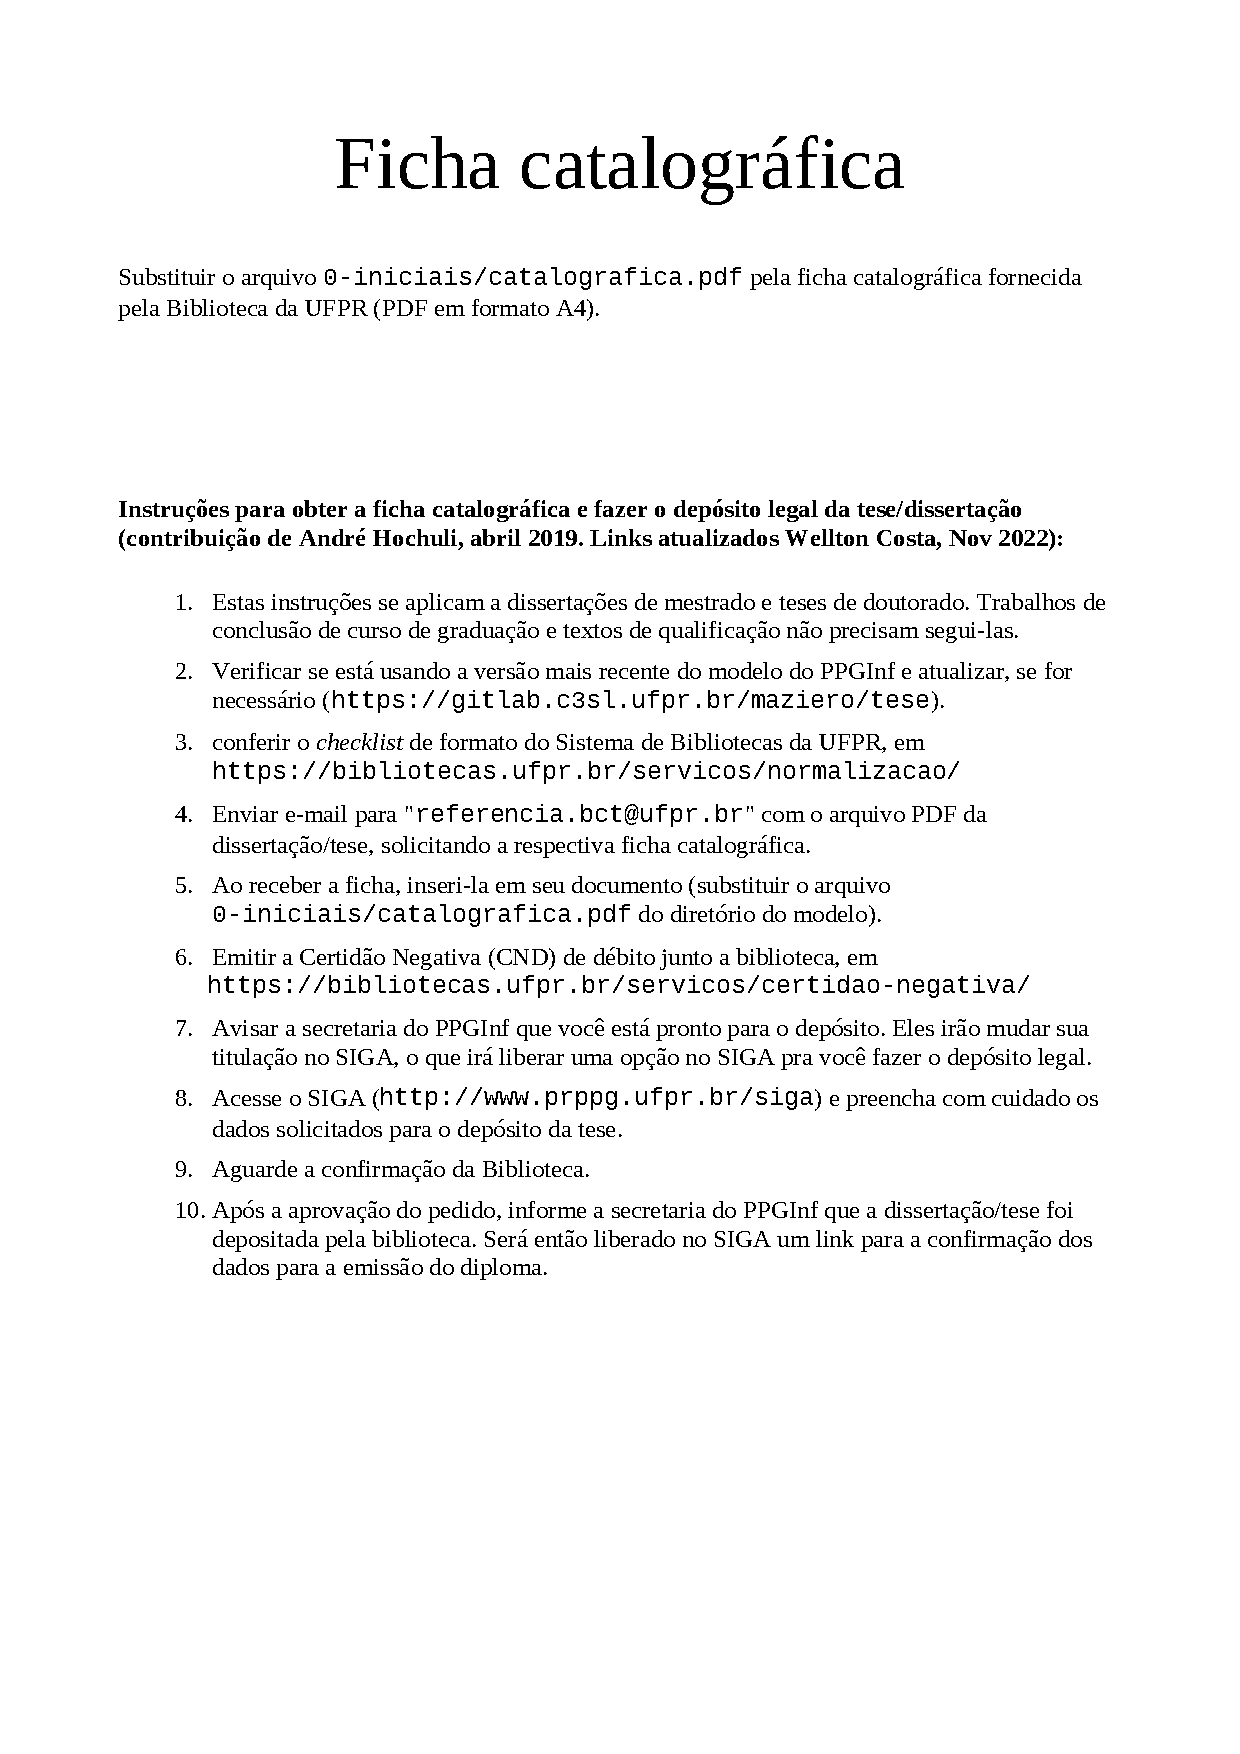
\includepdf[noautoscale]{0-iniciais/catalografica.pdf}

\end{ficha}

%=====================================================
	% ficha catalográfica
% A ficha de aprovação será fornecida pela secretaria do programa,
% após a defesa e cumprimento dos demais trâmites legais.

\begin{aprovacao}	% só gera conteúdo se for na versão final

% inclusão do termo de aprovação final (arquivo PDF)
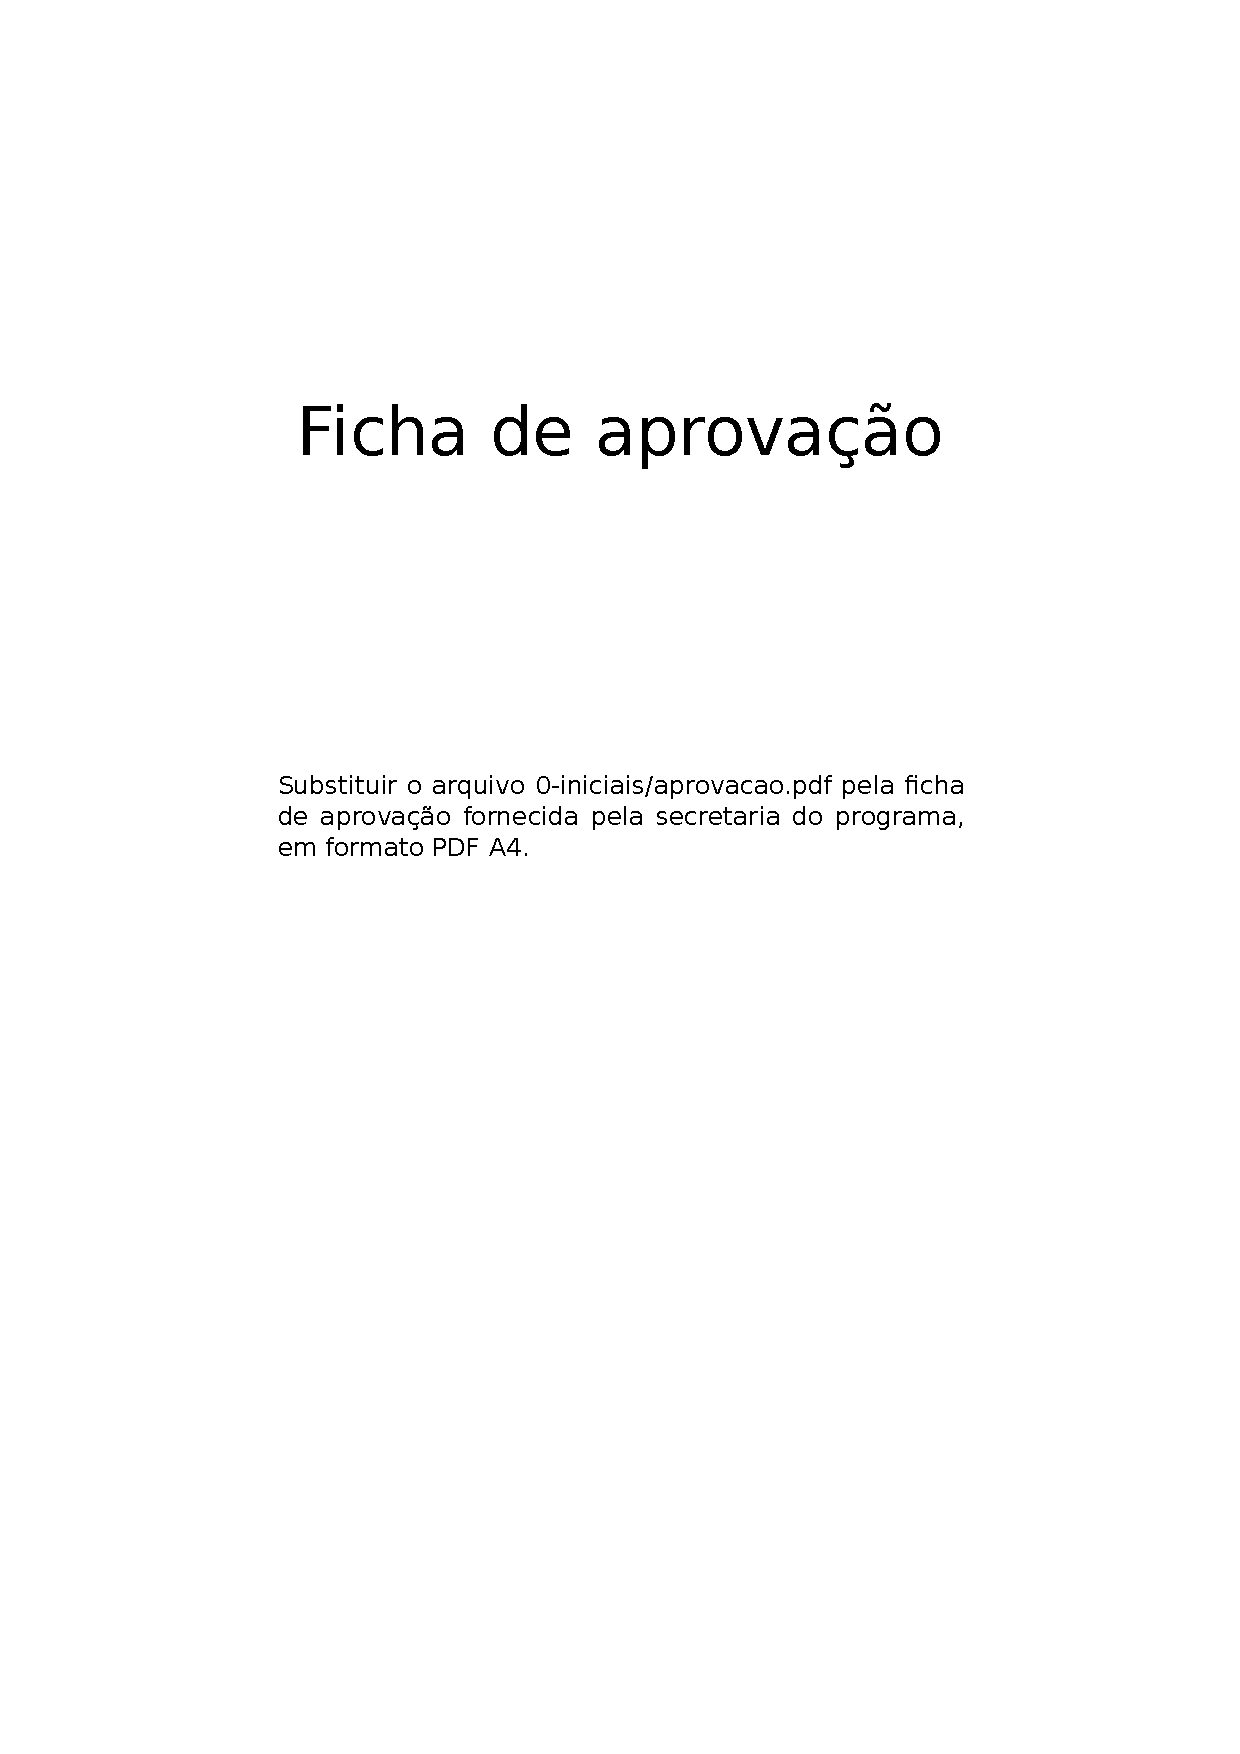
\includepdf[noautoscale]{0-iniciais/aprovacao.pdf}

\end{aprovacao}

%=====================================================
		% folha de aprovação
\begin{dedica}  % só gera conteúdo se for na versão final

"I see now that the circumstances of one's birth are irrelevant. It is what you do with the gift of life that determines who you are."
\begin{flushright}
--- Mewtwo
\end{flushright}

\end{dedica}

		% dedicatória
\begin{agradece}	% só gera conteúdo se for na versão final

Gostaria de expressar minha profunda gratidão ao Prof. Dr. Bruno Müller Jr., meu
orientador, por ter me emprestado de sua vasta experiência e por ter me guiado
com maestria em como escrever um artigo científico. Sinto-me verdadeiramente
honrado por ter sido orientado por ele em seu último ano como docente, antes de
sua merecida aposentadoria. Sua dedicação e conhecimento foram fundamentais para
o desenvolvimento deste trabalho.

Ao meu psicólogo Bruno Carvalho, agradeço por ter sido "coagido" a ler meus
rascunhos durante nossas sessões e, mesmo assim, ter me oferecido dicas valiosas
que contribuíram para o aprimoramento deste texto. Seu olhar diferenciado e
apoio foram essenciais durante este processo.

À minha mãe, agradeço por sempre ter insistido na importância de ter uma
educação superior. Sua determinação e incentivo foram a base que me permitiu
chegar até aqui.

A todos os participantes que aceitaram o convite para o experimento realizado
nesta pesquisa, minha sincera gratidão. Sem sua colaboração, este trabalho não
teria sido possível.

\end{agradece}

		% agradecimentos

% resumo (português) e abstract (inglês)
\begin{resumo}

Esta tese investiga o uso de bots como facilitadores de interações naturais em ambientes virtuais de ensino, visando viabilizar metodologias ativas no contexto remoto, considerando que a ausência de interações presenciais pode comprometer a eficácia de abordagens pedagógicas centradas no aluno. É explorado a definição e componentes de bots, suas aplicações educacionais e destaca três princípios fundamentais para interações mediadas: comunicação multidirecional, engajamento ativo e adaptação contextual. O trabalho apresenta o desenvolvimento de um bot educacional integrado ao Discord, plataforma escolhida por suas características que emulam um ambiente interativo, incluindo um dashboard exclusivo para professores que permite controle pedagógico não-invasivo e implementa recursos como feedback em tempo real, atividades colaborativas e ferramentas para aprendizagem baseada em problemas. A implementação técnica utiliza a biblioteca Concord em C, desenvolvida pelo autor, com arquitetura modular que gerencia publicação de conteúdo, interações, análise de dados e persistência. A prova de conceito demonstra funcionalidades como publicação estruturada, mecanismos de feedback rápido e coleta anônima de dúvidas, propondo uma metodologia de avaliação baseada em questionários, logs automáticos e entrevistas para mensurar engajamento, impacto pedagógico, usabilidade e viabilidade de implementação de metodologias ativas, concluindo que bots educacionais podem efetivamente aproximar o ambiente virtual da espontaneidade das interações presenciais, elemento fundamental para o sucesso das metodologias ativas no ensino remoto.

\end{resumo}

\begin{abstract}

This thesis investigates the use of bots as facilitators of natural interactions in virtual learning environments, aiming to enable active methodologies in remote teaching contexts, considering that the absence of face-to-face interactions can compromise the effectiveness of student-centered pedagogical approaches. It explores the definition and components of bots, their educational applications, and highlights three fundamental principles for mediated interactions: multidirectional communication, active engagement, and contextual adaptation. The work presents the development of an educational bot integrated with Discord, a platform chosen for its features that emulate an interactive environment, including an exclusive dashboard for teachers that allows non-invasive pedagogical control and implements resources such as real-time feedback, collaborative activities, and tools for problem-based learning. The technical implementation uses the Concord library in C, developed by the author, with a modular architecture that manages content publication, interactions, data analysis, and persistence. The proof of concept demonstrates functionalities such as structured publication, quick feedback mechanisms, and anonymous question collection, proposing an evaluation methodology based on questionnaires, automatic logs, and interviews to measure engagement, pedagogical impact, usability, and feasibility of implementing active methodologies, concluding that educational bots can effectively bring the virtual environment closer to the spontaneity of face-to-face interactions, a fundamental element for the success of active methodologies in remote teaching.    

\end{abstract}


% listas  de figuras, tabelas, abreviações/siglas, símbolos
\listoffigures				% figuras
\clearpage
\listoftables				% tabelas
%=====================================================

% lista de acrônimos (siglas e abreviações)

\begin{listaacron}

\begin{longtable}[l]{p{0.2\linewidth}p{0.7\linewidth}}
UI & \it{User Interface}\\
NLU & \it{Natural Language Understanding}\\
DM & \it{Dialogue Manager}\\
RG & \it{Response Generation}\\
API & \it{Application Programming Interface}\\
IHC & Interação Humano-Computador\\
MOOCs & \it{Massive Open Online Courses}\\
CRM & \it{Customer Relationship Management}\\
\end{longtable}

\end{listaacron}

%=====================================================
		% acrônimos, deve ser preenchida à mão
% %=====================================================

% lista de símbolos

\begin{listasimb}

\begin{longtable}[l]{p{0.2\linewidth}p{0.7\linewidth}}
$\alpha$ & alfa, primeira letra do alfabeto grego\\
$\beta$ & beta, segunda letra do alfabeto grego\\
$\gamma$ & gama, terceira letra do alfabeto grego\\
$\omega$ & ômega, última letra do alfabeto grego\\
$\pi$ & pi \\
$\tau$ & Tempo de resposta do sistema\\
$\theta$ & Ângulo de incidência do raio luminoso\\
\end{longtable}

\end{listasimb}

%=====================================================
		% símbolos, idem
\tableofcontents			% sumário

%=====================================================

% define estilo do corpo do documento (capítulos e apêndices)
\mainmatter
\pagestyle{mainmatter}

% inclusao de cada capítulo, alterar a gosto (do professor de Metodologia)
\chapter{Introdução}

%=====================================================

O ensino remoto tem se consolidado como uma alternativa viável para a disseminação do conhecimento, especialmente em cenários que exigem distanciamento social \cite{fabiane2024}. No entanto, essa modalidade apresenta desafios significativos, como a manutenção do engajamento dos alunos e a efetividade da comunicação entre docentes e discentes. A ausência de interações presenciais pode levar a uma experiência educacional menos dinâmica e participativa, distanciando as práticas pedagógicas de uma comunicação natural e espontânea \cite{fabiane2024}.

As metodologias ativas \cite{prince2004} de aprendizagem representam uma abordagem educacional que coloca o aluno como protagonista do processo de aprendizagem, em contraste com o ensino tradicional onde o estudante assume um papel predominantemente passivo. Estas metodologias envolvem participação direta, reflexão contínua e engajamento prático do aluno na construção do conhecimento. No contexto presencial, técnicas como aprendizagem baseada em problemas \cite{yew2016}, sala de aula invertida \cite{vanalten2019} e aprendizagem colaborativa \cite{laal2012} já demonstraram resultados positivos. No entanto, sua aplicação em ambientes remotos permanece um desafio significativo devido às limitações de interação natural entre os participantes \cite{fabiane2024}.

A integração de tecnologias interativas no ambiente educacional virtual emerge como elemento essencial para superar os obstáculos do ensino remoto e viabilizar metodologias ativas neste contexto. Dentre essas ferramentas capazes de recriar os elementos de metodologias ativas, estão os bots. Os bots, programas de computador capazes de simular interações humanas de forma automatizada e personalizada, apresentam-se como ferramentas capazes de recriar elementos de naturalidade na comunicação digital, aproximando o ambiente virtual da espontaneidade característica das interações presenciais \cite{okonkwo2021}.

Este trabalho tem como objetivo investigar o uso de bots como facilitadores de interações naturais em ambientes virtuais, o que poderia viabilizar a aplicação de metodologias ativas no ensino remoto. A pesquisa parte da observação que os bots podem atuar como pontes tecnológicas que diminuem a distância comunicativa entre participantes em ambientes virtuais, promovendo um fluxo mais natural e espontâneo de interações entre professores e alunos, sem que isso represente uma sobrecarga adicional para os docentes.

Para alcançar este objetivo, foi desenvolvido um bot integrado ao Discord, uma plataforma de comunicação virtual que, embora não seja tradicionalmente educacional, foi escolhida por oferecer recursos que emulam eficientemente um ambiente de ensino interativo. A plataforma suporta videoconferência, chat simultâneo, compartilhamento de conteúdo e criação de enquetes, proporcionando um ecossistema digital onde interações naturais podem ser facilitadas por um bot que intermedia as interações entre professor e aluno.

A pesquisa busca analisar como este bot pode criar um ambiente virtual onde interações naturais são facilitadas, tornando viável a aplicação de princípios de ensino ativo mesmo à distância. O estudo examina especificamente como esta ferramenta pode transformar a natureza das comunicações digitais educacionais, aproximando-as da fluidez e espontaneidade das interações presenciais, elementos fundamentais para o sucesso das metodologias ativas.

A eficácia da ferramenta é avaliada em três dimensões principais: o aumento do engajamento espontâneo dos alunos durante as aulas remotas, a fluidez e naturalidade da comunicação entre docentes e discentes mediada pelo bot, e a receptividade dos usuários quanto à integração dessa tecnologia como elemento natural do processo educacional.

O efeito do uso do bot proposto foi avaliado através da coleta de dados via preenchimento de questionários enviados aos participantes, e de informações extraídas pelo bot em sua mediação das interações básicas durante a experiência prática.

Este trabalho está organizado da seguinte forma: o Capítulo 2 apresenta a revisão bibliográfica, abordando conceitos fundamentais sobre bots, interações naturais e metodologias ativas em ambientes virtuais; o Capítulo 3 descreve a concepção e implementação do bot educacional proposto, com foco nas funcionalidades que promovem interações naturais; o Capítulo 4 detalha a prova de conceito e analisa os resultados obtidos no ambiente educacional remoto; e o Capítulo 5 apresenta a conclusão com análise dos resultados, limitações do estudo e sugestões de trabalhos futuros.

%=====================================================
			% introdução
\chapter{Revisão Bibliográfica}
\label{cap:revisao}

\graphicspath{\currfiledir/figuras/} % caminho para as figuras deste capítulo

%=====================================================

Este capítulo apresenta uma revisão da literatura sobre bots, seu uso em contextos educacionais e as tecnologias relacionadas ao seu desenvolvimento, estabelecendo as bases conceituais para este trabalho.

O Capítulo está organizado da seguinte forma: a Seção \ref{sec:def-bots} apresenta a definição e componentes de bots, a Seção \ref{sec:class-bots} discute as classificações de bots, a Seção \ref{sec:bots-educ} aborda os bots no contexto educacional, incluindo os desafios do ensino remoto e aspectos de interação humano-computador na educação, a Seção \ref{sec:ferramentas} analisa bibliotecas e tecnologias para desenvolvimento de bots, a Seção \ref{sec:trab-rel} apresenta trabalhos relacionados, e finalmente, a Seção \ref{sec:objetivos} delineia os objetivos específicos deste trabalho com base nos conceitos apresentados.

%=====================================================

\section{Definição e Componentes de Bots}
\label{sec:def-bots}

Bots são programas automatizados projetados para interagir com usuários ou sistemas, realizando tarefas específicas com diferentes níveis de autonomia. Bots podem ser definidos como "aplicações que combinam uma interface conversacional com a capacidade de executar tarefas específicas para o usuário" \cite{dale2016}, ou também "uma aplicação que realiza certas tarefas repetitivas de maneira mais rápida que o ser humano" \cite{eslahi2012}.

A arquitetura de um bot pode ser descrita de diferentes maneiras na literatura, mas geralmente envolve um conjunto de componentes essenciais que trabalham juntos para processar a entrada do usuário, gerenciar o diaĺogo e gerar respostas apropriadas. Uma estrutura comum inclui como elementos principais (1) interface do usuário, (2) compreensão de linguagem natural, (3) gerenciador de diálogo, (4) integração com backend, e por fim (5) geração de linguagem natural \cite{huang2021}:

\begin{enumerate}
\item \textbf{Interface do Usuário (User Interface - UI)}: Este é o ponto de contato entre o usuário e o bot. A UI é responsável por receber a entrada do usuário (texto, voz, cliques em elementos gráficos) e apresentar as respostas do bot de forma compreensível. Pode variar desde simples janelas de chat baseadas em texto até interfaces de voz sofisticadas ou GUIs interativas.
\item \textbf{Compreensão de Linguagem Natural (Natural Language Understanding - NLU)}: Este componente é crucial para interpretar a entrada do usuário em linguagem natural. Ele analisa o texto ou a fala para identificar a intenção do usuário (o que o usuário quer fazer) e extrair informações relevantes, conhecidas como entidades (por exemplo, datas, locais, nomes). O NLU transforma a entrada não estruturada do usuário em dados estruturados que o bot pode processar.
\item \textbf{Gerenciador de Diálogo (Dialogue Manager - DM)}: O DM mantém o estado do diálogo (o contexto da conversa), rastreia o histórico de interações e decide qual ação tomar a seguir com base na intenção identificada pelo NLU e nas regras de negócio ou na lógica conversacional definida. Isso pode envolver fazer perguntas de esclarecimento, acessar a base de conhecimento, chamar uma API externa ou gerar uma resposta. O DM pode ser implementado usando abordagens baseadas em regras ou modelos de aprendizado de máquina mais complexos.
\item \textbf{Integração com Backend e Base de Conhecimento (Backend Integration \& Knowledge Base)}: Para realizar tarefas úteis e fornecer informações precisas, os chatbots frequentemente precisam interagir com sistemas externos e acessar dados. A integração com o backend permite que o bot se conecte a APIs, bancos de dados, sistemas de CRM, ou outras fontes de informação e serviços. Essa base de conhecimento pode incluir conhecimento estático (pré-programado), conhecimento dinâmico (acessado em tempo real via APIs), conhecimento contextual (histórico do usuário) e até conhecimento colaborativo (gerado pelo usuário). É importante a integração com o backend para acessar essas informações e executar ações.
\item \textbf{Geração de Resposta (Response Generation - RG)}: Uma vez que o Gerenciador de Diálogo decide a resposta a ser dada, o componente RG a transforma em linguagem natural (texto ou fala) para ser apresentada ao usuário através da Interface do Usuário. A complexidade do RG pode variar desde o uso de modelos de resposta pré-definidos até a geração dinâmica de sentenças complexas.
\end{enumerate}

\begin{figure}[!htb]
\centering
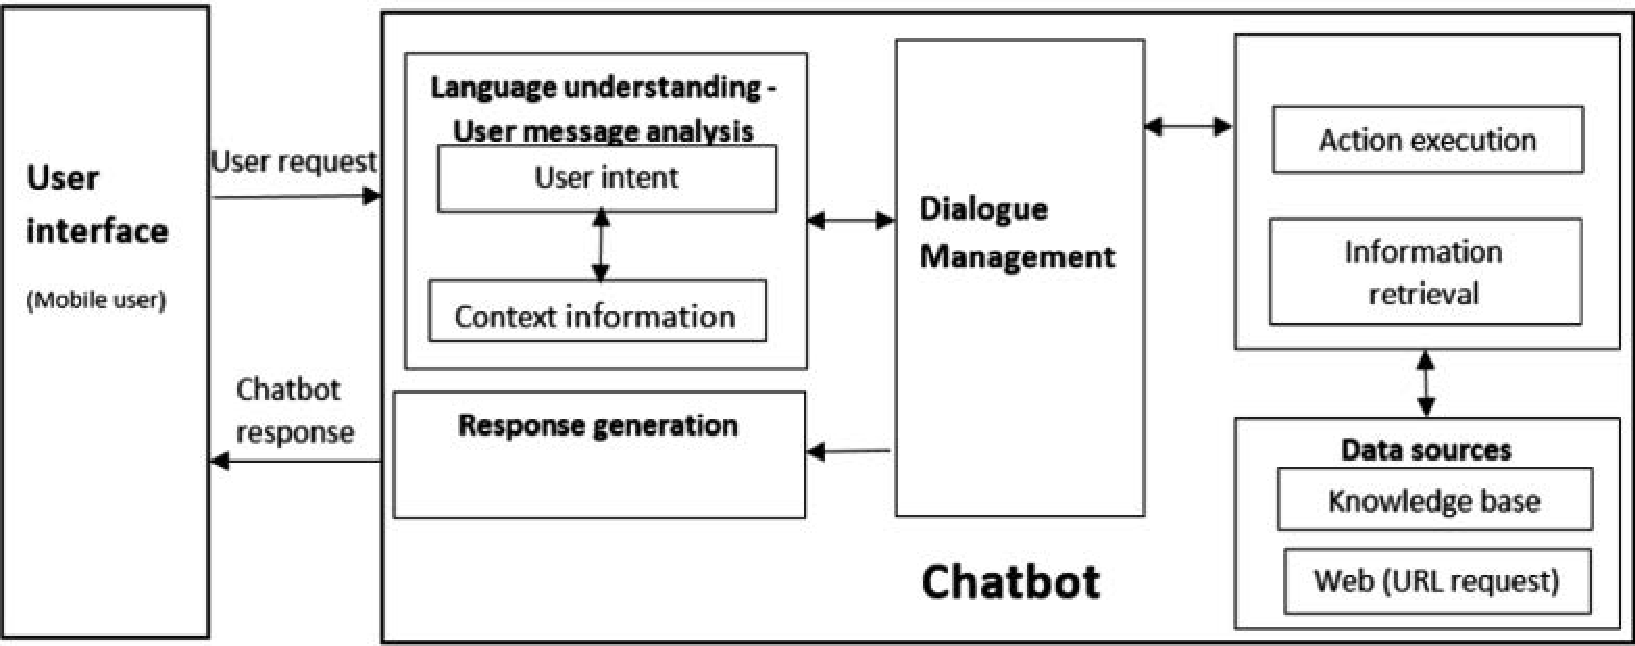
\includegraphics[width=12cm]{huang-arquitetura.pdf}
\caption{Arquitetura de um chatbot por Huang et al. \cite{huang2021}.}
\label{fig:bot-arch}
\end{figure}


%=====================================================

\section{Classificações de Bots}
\label{sec:class-bots}

Existem diversas formas de classificar bots, dependendo de suas características, funcionalidades e aplicações. Os bots podem ser classificados de acordo com seu propósito principal \cite{lebeuf2019}, ou de acordo com a sua funcionalidade primária \cite{seering2018}.

\begin{table}[H]
\centering
\label{tab:classificacao_bots}
\begin{tabular}{|p{4.2cm}|p{9cm}|}
\hline
\textbf{Propósito}\cite{lebeuf2019}& \textbf{Descrição} \\
\hline
Bots generalistas & Executam uma ampla variedade de tarefas, como responder perguntas gerais e executar comandos simples. \\
\hline
Bots transacionais & Realizam transações com sistemas externos, como bots bancários ou de compras. \\
\hline
Bots informacionais & Fornecem informações e respondem perguntas específicas dos usuários. \\
\hline
Bots de produtividade & Automatizam tarefas repetitivas, como lembretes ou agendamentos. \\
\hline
Bots de colaboração & Facilitam a interação e colaboração entre usuários, geralmente em ambientes de comunicação. \\
\hline
\textbf{Funcionalidade}\cite{seering2018} & \textbf{Descrição} \\
\hline
Tarefas administrativas & Auxiliam na organização de atividades, como agendar reuniões e gerenciar compromissos. \\
\hline
Entretenimento & Proporcionam atividades lúdicas, como jogos ou interações divertidas. \\
\hline
Funcionalidade e qualidade & Aumentam a eficiência de serviços, como bots de suporte técnico ou de coleta de feedback. \\
\hline
Comunidade & Moderam e gerenciam interações em comunidades online. \\
\hline
Arquivadores & Organizam e recuperam informações, como documentos e registros de mensagens. \\
\hline
\end{tabular}
\caption{Classificação de bots segundo propósito e funcionalidade}
\end{table}

\noindent Este trabalho concentra-se em bots do tipo "produtividade" e "colaboração" como propósito, e "funcionalidade e qualidade" como funcionalidade. O foco é a sua aplicação dentro do contexto educacional, onde eles podem atuar como assistentes virtuais que facilitam a interação entre alunos e professores, a fim de promover um ambiente remoto de aprendizagem mais dinâmico e interativo.

%=====================================================

\section{Bots no Contexto Educacional}
\label{sec:bots-educ}

Na educação, os bots têm sido utilizados para diversos propósitos, desde fornecer suporte administrativo até oferecer experiências de aprendizado personalizadas. Os bots educacionais podem transformar a experiência de aprendizagem ao oferecer suporte contínuo e personalizado que seria impraticável para um professor humano fornecer a todos os alunos simultaneamente \cite{zawacki2019}.

Estudos recentes têm explorado aplicações educacionais específicas de bots. Por exemplo, o uso de chatbots para melhorar a retenção de conhecimento em estudantes universitários \cite{okonkwo2021}, e aumentar o engajamento em cursos online abertos e massivos (MOOCs) \cite{han2022}.

De uma maneira geral, bots educacionais são particularmente eficazes quando (1) fornecem feedback imediato aos alunos, (2) oferecem disponibilidade contínua para assistência, (3) personalizam a experiência de aprendizado, (4) reduzem a carga cognitiva dos instrutores e (5) permitem que os instrutores se concentrem em atividades pedagógicas e interativas \cite{silva2024}.

A seguir, exploramos quatro dimensões importantes relacionadas ao uso de bots educacionais: os desafios específicos do ensino remoto que podem ser mitigados por essas ferramentas, os princípios de interação humano-computador relevantes para o design de bots educacionais eficazes, os princípios fundamentais para a interação mediada por bots na educação, e o papel dos dashboards como ferramentas de controle pedagógico.

%-----------------------------------------------------

\subsection{Desafios do Ensino Remoto}
\label{subsec:desafios}

O ensino remoto apresenta desafios únicos que podem ser parcialmente mitigados pelo uso de tecnologias interativas como bots. Aqui se faz distinção entre "ensino remoto emergencial" e educação online planejada, destacando que muitas instituições foram forçadas a adotar o primeiro modelo durante a pandemia de COVID-19, sem tempo adequado para planejamento \cite{hodges2020}\cite{fabiane2024}.

\noindent Entre os principais desafios identificados estão \cite{fabiane2024}:

\begin{itemize}
\item Limitações tecnológicas e acesso desigual
\item Competências digitais insuficientes de professores e alunos
\item Falta de estrutura para avaliação eficaz
\item Dificuldade em manter o engajamento dos alunos
\item Ausência de interação social e senso de comunidade
\end{itemize}

\noindent Tecnologias como bots podem preencher algumas dessas lacunas ao proporcionar uma interface natural e contínua entre os participantes do processo educacional, oferecendo um canal adicional de comunicação e suporte tanto para alunos quanto para professores \cite{winkler2018}.

%-----------------------------------------------------

\subsection{Interação Humano-Computador na Educação}
\label{subsec:ihc}

Estudos em IHC destacam a importância de sistemas que se ajustem ao comportamento e às necessidades dos usuários \cite{roy1987}. Na educação, isso implica em promover interfaces que permitam participação ativa, acessibilidade e adaptabilidade aos estilos de aprendizagem dos alunos.

Norman \cite{norman2013} enfatiza o conceito de design centrado no usuário, onde a tecnologia deve se adaptar às necessidades humanas e não o contrário. Aplicado ao contexto educacional, este princípio sugere que os bots devem ser projetados considerando as necessidades pedagógicas específicas e as limitações cognitivas dos alunos.

Bots educacionais se encaixam nesse contexto por serem acessíveis e flexíveis na forma de interação. Interfaces conversacionais podem reduzir a carga cognitiva associada à navegação em sistemas educacionais complexos, permitindo que os alunos se concentrem no conteúdo do aprendizado em vez de na interface \cite{sweller2011}.

%-----------------------------------------------------

\subsection{Princípios para Interação Mediada por Bots na Educação}
\label{subsec:principios}

Com base na literatura sobre bots educacionais e metodologias ativas, surgem três princípios fundamentais emergem como pilares para o design de interações eficazes mediadas por bots em ambientes educacionais:

\begin{enumerate}
\item \textbf{Comunicação multidirecional}: Um bot educacional eficaz não deve apenas transmitir informações do professor para os alunos, mas também facilitar o retorno dos alunos para o professor, criando um ciclo contínuo de feedback. Esse princípio alinha-se com a concepção de aprendizagem dialógica \cite{calvo2013}, onde o conhecimento é construído através da interação bidirecional entre educador e educando.
\item \textbf{Engajamento ativo}: Através de mecânicas interativas, o bot deve estimular constantemente a participação dos alunos, transformando-os de receptores passivos a agentes ativos no processo de aprendizagem. Este princípio está fundamentado nas teorias construtivistas de aprendizagem \cite{piaget1970}, que enfatizam a importância da experiência prática e da participação na construção do conhecimento.
\item \textbf{Adaptação contextual}: O sistema deve se ajustar ao ritmo da aula e às necessidades específicas da disciplina, oferecendo diferentes modos de interação conforme o momento pedagógico. Tecnologias educacionais eficazes devem ser flexíveis o suficiente para se adaptarem a diferentes contextos pedagógicos e estilos de aprendizagem \cite{winkler2018}.
\end{enumerate}

Estes princípios fornecem uma base teórica para o design de bots educacionais que efetivamente aprimoram o processo de aprendizagem, especialmente em contextos de metodologias ativas onde a participação e o engajamento dos alunos são essenciais.

%-----------------------------------------------------

\subsection{Dashboards como Ferramenta de Controle Pedagógico}
\label{subsec:dashboards}

Um elemento crucial no design de bots educacionais é a interface de controle que permite aos educadores gerenciar o fluxo das interações. Os dashboards pedagógicos surgem como uma solução para esta necessidade, oferecendo uma visão consolidada das atividades e permitindo intervenções em tempo real sem interromper o fluxo da aula \cite{verbert2013}.

Dashboards de aprendizagem são "displays únicos que agregam diferentes indicadores sobre aprendiz, atividades de aprendizagem e/ou contexto de aprendizagem em uma ou múltiplas visualizações" \cite{verbert2013}. No contexto de bots educacionais, estes dashboards evoluem para se tornarem não apenas ferramentas de visualização, mas interfaces de comando que permitem aos professores:

\begin{enumerate}
\item \textbf{Orquestrar atividades}: Iniciar e controlar sequências de aprendizagem sem necessidade de inserir comandos em chats públicos
\item \textbf{Monitorar em tempo real}: Visualizar métricas de engajamento e compreensão durante a aula
\item \textbf{Receber alertas}: Ser notificado sobre padrões que exijam intervenção pedagógica
\item \textbf{Personalizar interações}: Adaptar atividades com base nas necessidades observadas
\item \textbf{Analisar resultados}: Obter relatórios detalhados após as sessões
\end{enumerate}

\begin{figure}[H]
\centering
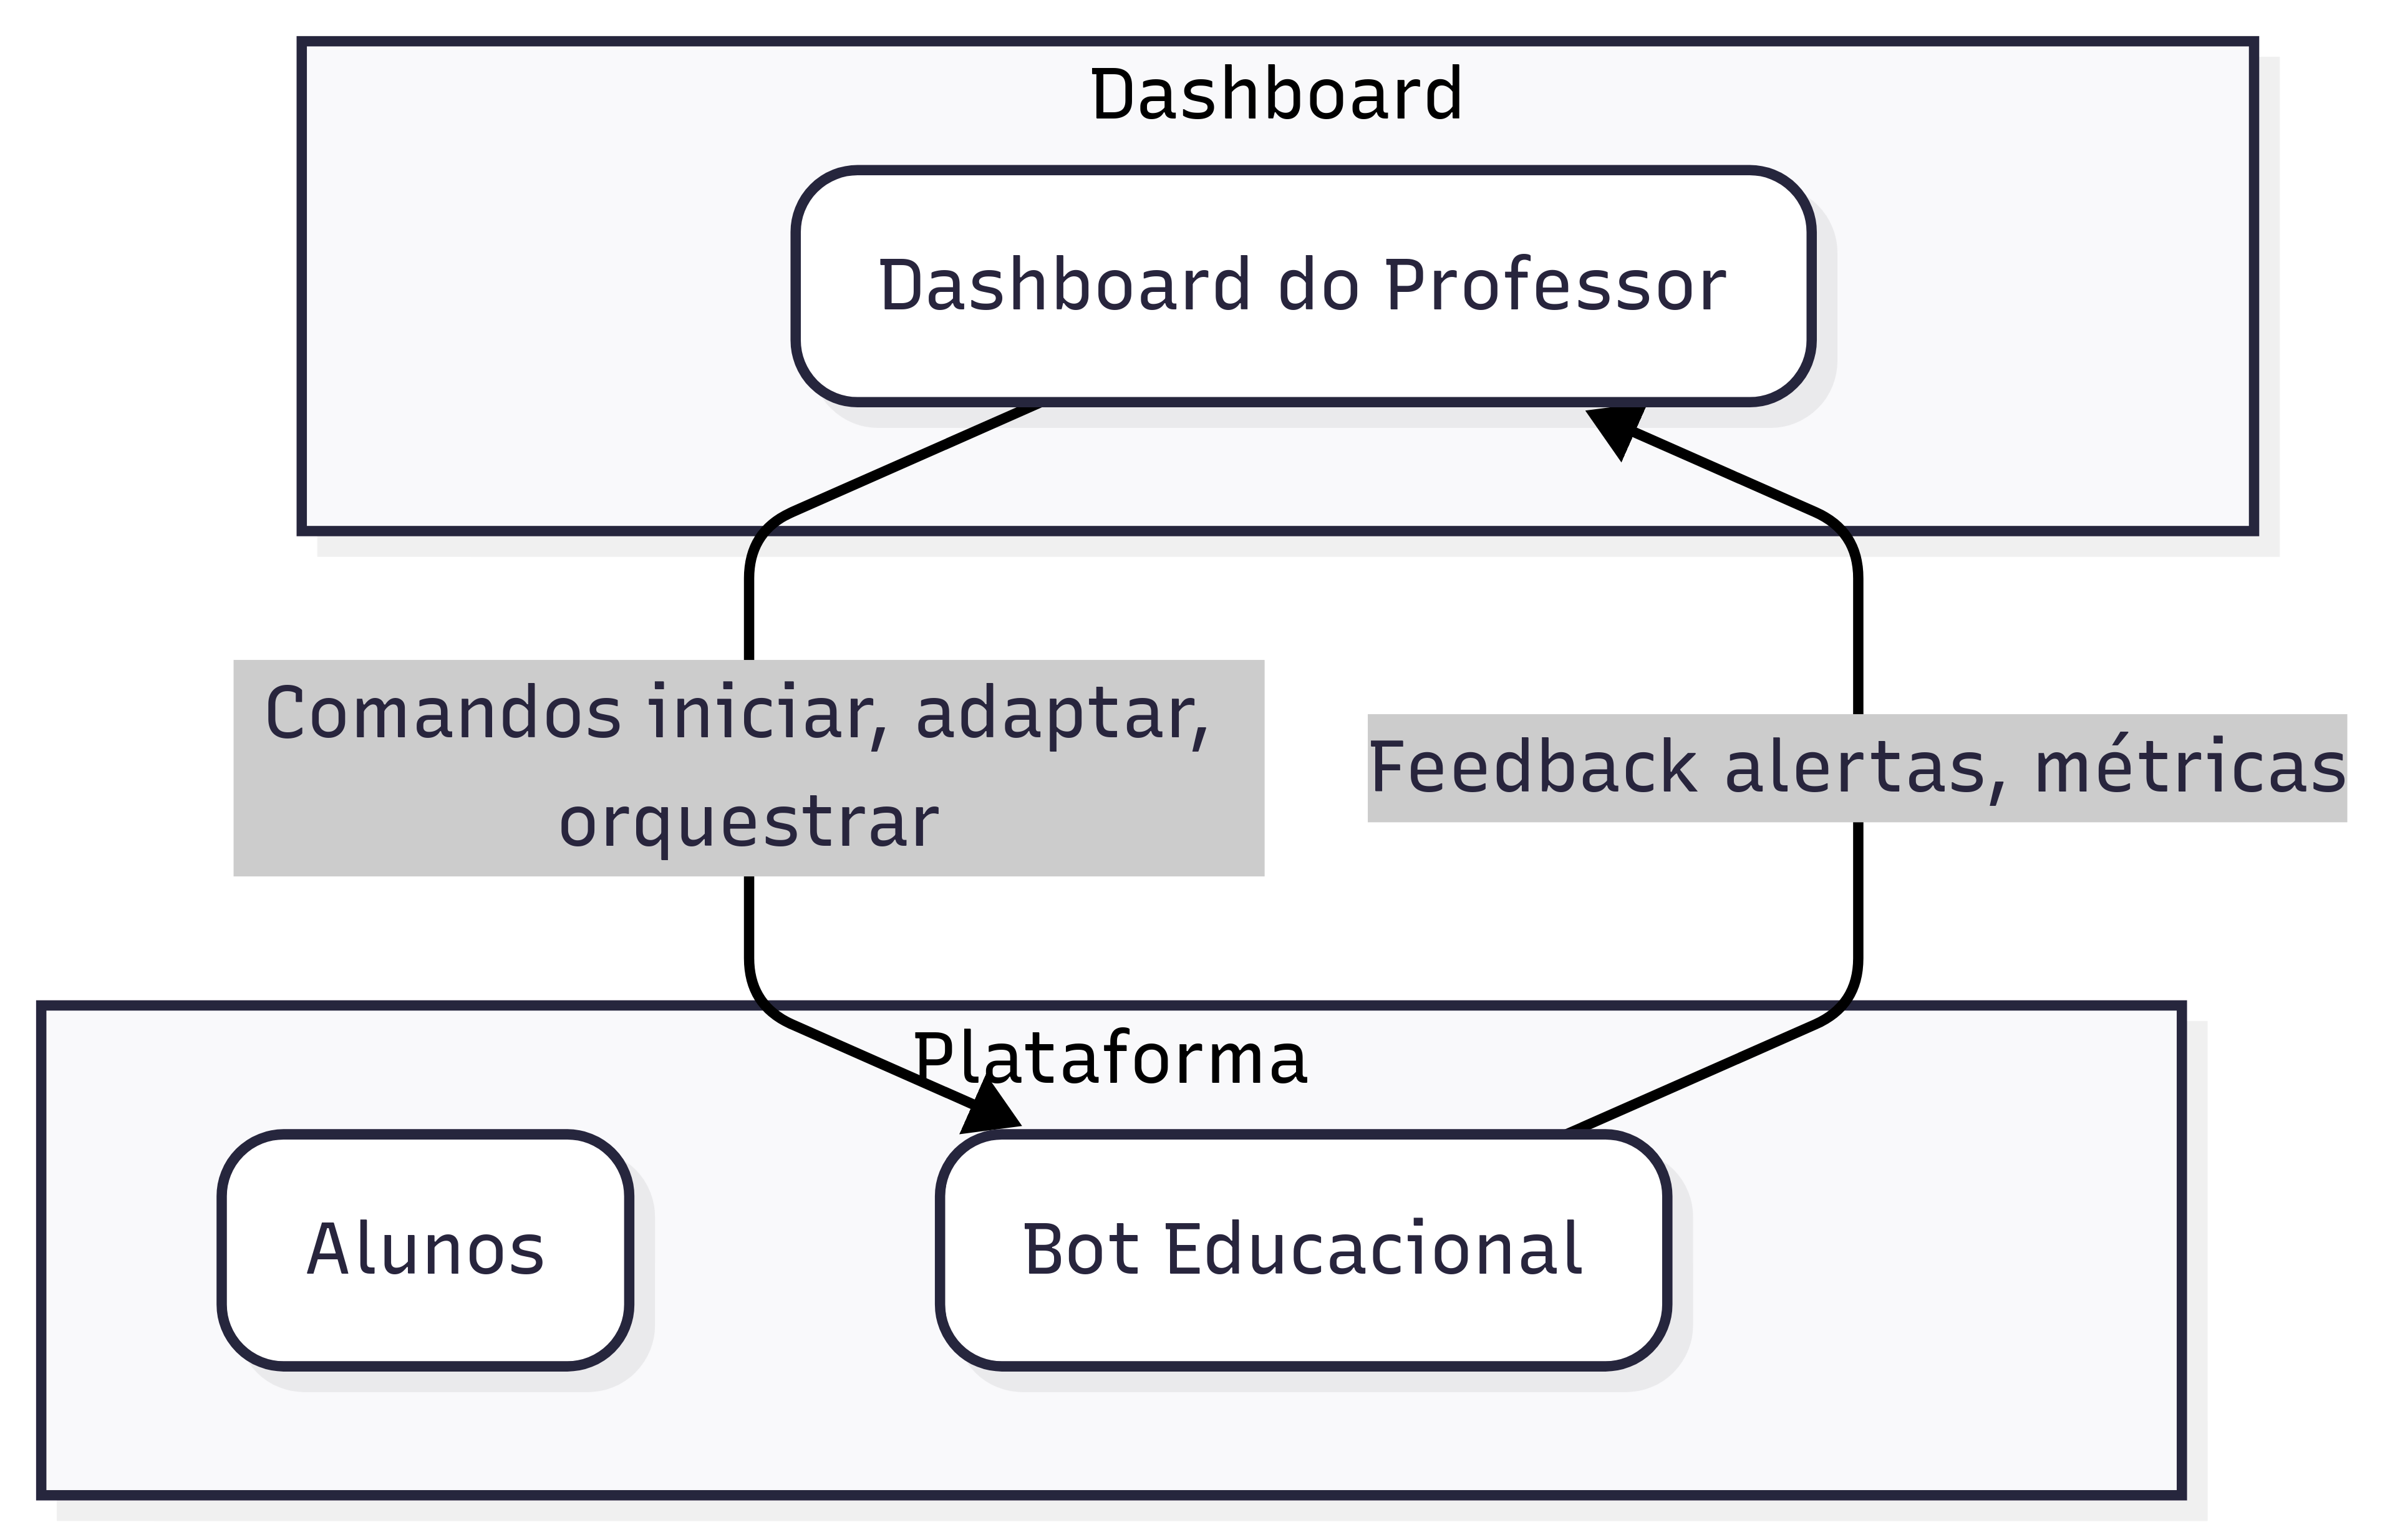
\includegraphics[width=12cm]{relacao-dashboard-bot.png}
\caption{Relação entre o bot educacional e o dashboard de controle pedagógico.}
\label{fig:dashboard-bot}
\end{figure}

Esta abordagem separa claramente o canal de comando (dashboard, visível apenas para o professor) do canal de interação (plataforma de comunicação, visível para todos os participantes), seguindo o princípio de "separação de interesses" como essencial para ambientes de aprendizagem tecnologicamente mediados. A eficácia desse modelo de interação será avaliada em experimentos controlados, onde participantes assumirão papéis de professor e alunos, interagindo em um ambiente de sala de aula simulado.

%=====================================================

\section{Ferramentas para Desenvolvimento de Bots no Discord}
\label{sec:ferramentas}

Existem várias ferramentas para desenvolver bots, dentre elas destacamos bibliotecas específicas para a plataforma do Discord, cada uma com suas particularidades e casos de uso apropriados, (1) JavaScript/Node.js, (2) Python e (3) C. 

\begin{enumerate}
\item \textbf{Discord.js}\cite{discordjs}: Uma biblioteca JavaScript/Node.js que oferece abstração de alto nível para interação com a API do Discord. É rica em recursos e possui uma comunidade ativa, sendo adequada para desenvolvedores que preferem desenvolvimento rápido.
\item \textbf{Discord.py}\cite{discordpy}: Equivalente ao Discord.js, mas para a linguagem Python. Oferece abstrações semelhantes e é amplamente utilizada para desenvolvimento de bots no Discord.
\item \textbf{Concord}\cite{muller}: Uma biblioteca em C que fornece acesso de baixo nível à API do Discord, desenvolvida pelo autor deste trabalho. Diferentemente das opções anteriores, a Concord prioriza desempenho e controle direto sobre a API, sendo apropriada para aplicações que demandam eficiência computacional e controle granular.
\end{enumerate}

No contexto deste estudo, foi escolhida a biblioteca Concord, por sua implementação na linguagem C, que oferece um equilíbrio entre abstração e controle que a torna adequada para uma ampla gama de aplicações \cite{kernighan1988}. No contexto educacional, C é frequentemente utilizada como linguagem de ensino em cursos de programação devido à sua sintaxe fundamental que expõe conceitos importantes de ciência da computação, como gerenciamento de memória e estruturas de dados básicas \cite{kernighan1988}.

Para estudos futuros, é importante considerar o uso de linguagens de mais alto nível como Python, JavaScript ou Go, que podem oferecer desenvolvimento mais rápido e maior facilidade de manutenção, especialmente em projetos onde a curva de aprendizado reduzida seja prioritária em relação ao desempenho bruto. A linguagem de programação em contextos educacionais deve equilibrar considerações pedagógicas, praticidade de implementação e objetivos específicos do projeto \cite{pears2007}.

%=====================================================

\section{Trabalhos Relacionados}
\label{sec:trab-rel}

Diversos pesquisadores têm explorado o uso de bots em contextos educacionais:

Hien et al. \cite{hien2018} desenvolveram um bot para suporte a alunos em um curso de programação, que respondia a dúvidas sobre conceitos e sintaxe. Os resultados mostraram uma redução no tempo de resposta para dúvidas comuns e um aumento na satisfação dos alunos com o suporte recebido.

Demetriadis et al. \cite{demetriadis2018} implementaram um agente conversacional para auxiliar alunos em atividades colaborativas de resolução de problemas. O estudo demonstrou que grupos apoiados pelo bot apresentaram maior engajamento e melhores resultados de aprendizagem em comparação com grupos sem suporte automatizado.

Yin et al. \cite{yin2024} compararam o fornecimento de feedback formativo aos alunos por chatbot e professor. A avaliação indicou que alunos que receberam feedback regularmente do chatbot apresentaram maior interesse de aprendizagem, além de redução da carga cognitiva necessária para aprender conceitos complexos.

Um trabalho particularmente relevante é o de Winkler e Söllner \cite{winkler2018}, que propõe diretrizes para o design de chatbots educacionais focados em metodologias ativas, destacando a importância de promover interações que estimulem o pensamento crítico e a reflexão.

%=====================================================

\section{Objetivos do Trabalho}
\label{sec:objetivos}

Com base na revisão bibliográfica apresentada, este trabalho tem como objetivo desenvolver e avaliar um bot educacional assistivo e conversacional para plataformas de colaboração, especificamente o Discord, que facilite a implementação de metodologias ativas em ambientes de ensino remoto.

Os objetivos específicos incluem:

\begin{enumerate}
\item \textbf{Desenvolver um bot educacional} que incorpore os três princípios fundamentais para interação mediada discutidos na Seção \ref{subsec:principios}: comunicação multidirecional, engajamento ativo e adaptação contextual.
\item \textbf{Implementar funcionalidades específicas} que abordem diretamente os desafios do ensino remoto identificados na Seção \ref{subsec:desafios}, com foco especial em manter o engajamento dos alunos, facilitar o feedback imediato e promover interações sociais significativas em ambientes virtuais.
\item \textbf{Proporcionar uma integração não-invasiva} da ferramenta ao fluxo de trabalho docente, aplicando os princípios de design centrado no usuário e minimizando a carga cognitiva adicional, conforme destacado nos estudos de IHC educacional na Seção \ref{subsec:ihc}.
\item \textbf{Criar uma prova de conceito funcional} utilizando tecnologias adequadas ao contexto educacional, considerando aspectos de eficiência, portabilidade e manutenção, conforme discutido na Seção \ref{sec:ferramentas}.
\item \textbf{Estabelecer uma metodologia de avaliação experimental} com participantes reais assumindo os papéis de professor e alunos, onde o professor utiliza o dashboard de controle enquanto os alunos interagem com o bot em um ambiente de sala de aula simulado, permitindo mensurar a eficácia da solução em situações próximas ao uso real, combinando métricas quantitativas e qualitativas, inspirada nos trabalhos apresentados na Seção \ref{sec:trab-rel}.
\end{enumerate}

Tecnicamente, o desenvolvimento será realizado utilizando a biblioteca Concord em C (desenvolvida pelo autor), aproveitando suas vantagens em termos de controle granular sobre a API do Discord e sua relevância educacional, conforme discutido na Seção \ref{sec:ferramentas}.

Este trabalho se diferencia dos esforços anteriores apresentados na Seção \ref{sec:trab-rel} por seu foco específico em facilitar metodologias ativas em ambientes remotos, com ênfase na integração não-invasiva à prática docente e sua metodologia de avaliação que simula condições reais de uso. Enquanto outros trabalhos têm explorado bots para responder dúvidas ou fornecer feedback automatizado, esta proposta busca transformar a própria dinâmica de interação durante as aulas síncronas, com uma avaliação sistemática em um ambiente controlado.

Os próximos capítulos detalham a concepção e implementação do bot (\ref{cap:bot}), bem como sua avaliação através da metodologia experimental com participantes em diferentes papéis (Capítulo 4), demonstrando como os conceitos teóricos discutidos neste capítulo se manifestam na prática educacional.		% fundamentação teórica
\chapter{Bot Educacional para Metodologias Ativas em Ambientes Virtuais}
\label{cap:bot}

% Usar o graphicspath para buscar figuras no subdiretório figuras
\graphicspath{\currfiledir/figuras/}

%=====================================================

Este capítulo apresenta a concepção do bot educacional desenvolvido neste trabalho, sua arquitetura funcional e como ele se integra ao ambiente de ensino remoto para facilitar metodologias ativas. Para ilustrar a aplicação prática, utilizaremos um exemplo concreto baseado em uma aula de programação da disciplina CI1055 - Algoritmos e Estruturas de Dados I.

%=====================================================

\section{Visão Conceitual da Aplicação}
\label{sec:visao}

O bot educacional proposto foi concebido como um mediador de interações em ambientes virtuais de aprendizagem, especificamente voltado para facilitar a implementação de metodologias ativas durante sessões de ensino remoto. O sistema atua como uma ponte entre professor e alunos, promovendo trocas mais naturais de informações e feedback.

A Figura a seguir ilustra o modelo conceitual de interação entre os participantes do processo educacional mediado pelo bot:

\begin{figure}[htb]
\centering
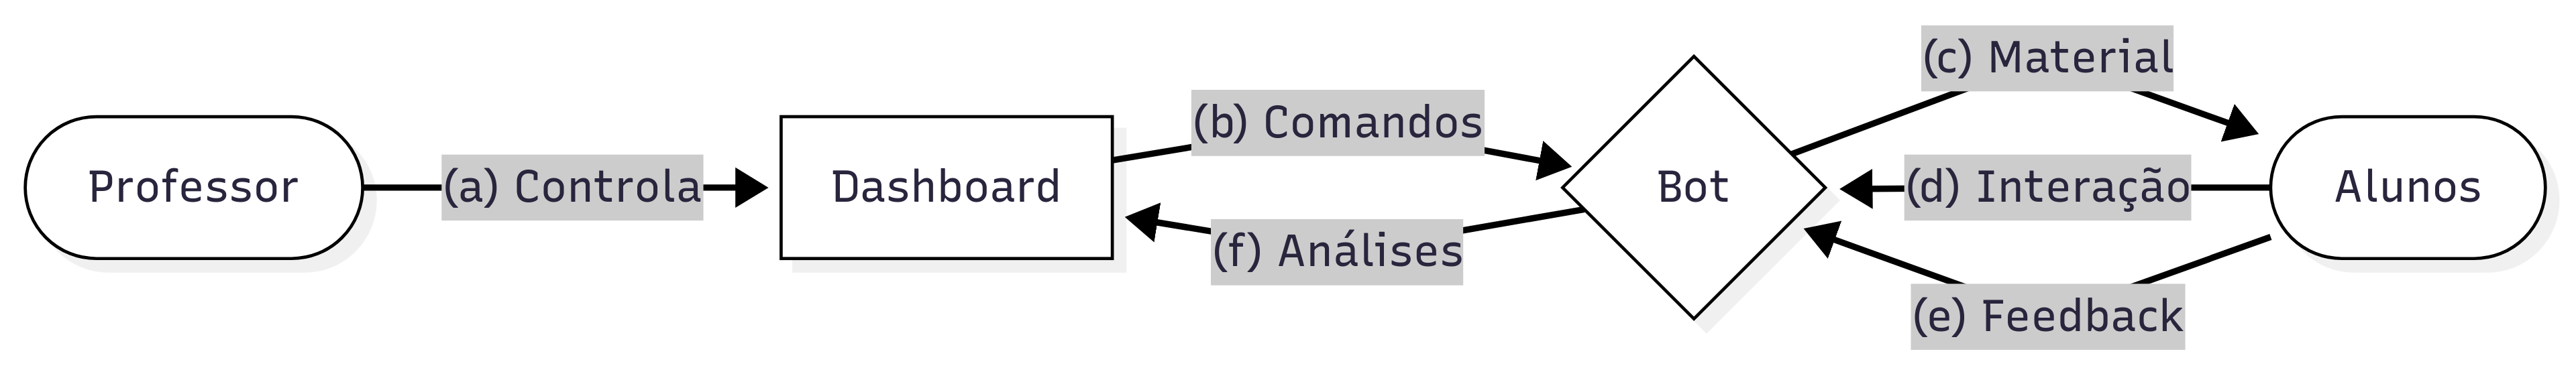
\includegraphics[width=12cm]{modelo-interacao.png}
\caption{Fluxo de interações no ambiente educacional virtual mediado pelo bot. A figura mostra um diagrama com o professor à esquerda, o dashboard do professor como interface de controle, o bot educacional ao centro, e os alunos à direita, ilustrando os fluxos de comunicação: (a) professor controlando a aula via dashboard, (b) dashboard enviando comandos ao bot, (c) bot processando e disponibilizando o material para os alunos, (d) alunos interagindo com o conteúdo, (e) bot coletando feedback dos alunos, e (f) bot fornecendo análises em tempo real ao professor através do dashboard.} 
\label{fig:modelo-interacao}
\end{figure}

O modelo de interação implementado neste trabalho fundamenta-se nos três princípios para interação mediada por bots na educação discutidos na Seção \ref{subsec:principios}: comunicação multidirecional, engajamento ativo e adaptação contextual. Estes princípios nortearam todo o processo de design e desenvolvimento da solução, garantindo que o bot efetivamente contribua para a implementação de metodologias ativas no ambiente virtual.

%=====================================================

\section{Integração com o Ambiente Educacional}
\label{sec:integracao}

O bot foi projetado para se integrar ao Discord, uma plataforma de comunicação digital que combina recursos de chat em texto, voz e compartilhamento de mídia. Embora o Discord tenha sido originalmente desenvolvido para comunidades de jogos, as seguintes características o tornam adequado para emular um ambiente educacional remoto:

\begin{itemize}
\item \textbf{Canais temáticos}: Permitem organizar discussões por tópicos específicos
\item \textbf{Transmissão de voz/vídeo}: Facilita aulas síncronas com interação audiovisual
\item \textbf{Compartilhamento de tela}: Possibilita demonstrações práticas pelo professor
\item \textbf{Sistema de reações}: Oferece mecanismo não-verbal para expressão de compreensão ou dúvidas
\item \textbf{Persistência de mensagens}: Mantém o histórico de interações disponível para consulta posterior
\end{itemize}

A \textbf{integração sutil} com o ambiente educacional, refere-se à capacidade do bot de participar do processo educacional sem causar rupturas no fluxo natural da aula ou exigir mudanças drásticas nas práticas pedagógicas já estabelecidas. Essa sutileza manifesta-se em três dimensões:

\begin{enumerate}
\item \textbf{Presença não-intrusiva}: O bot não interrompe a condução da aula, apenas complementa as atividades quando solicitado ou programado.
\item \textbf{Curva de aprendizado reduzida}: Professores e alunos não precisam dominar ferramentas complexas, pois as interações ocorrem através de comandos intuitivos e reações simples.
\item \textbf{Flexibilidade metodológica}: O sistema adapta-se a diferentes estilos de ensino, não impondo uma abordagem pedagógica específica.
\end{enumerate}

Para materializar esta integração, o sistema também disponibiliza um dashboard específico para uso do professor, que permite o controle da aula de forma centralizada e intuitiva, sem a necessidade de comandos complexos ou interrupções no fluxo de comunicação, como será detalhado na seção \ref{subsec:dashboard}.

%-----------------------------------------------------

\subsection{Dashboard do Professor}
\label{subsec:dashboard}

Um elemento chave do sistema é o dashboard exclusivo para o professor, que permite controlar o fluxo da aula sem a necessidade de inserir comandos no chat principal. Este dashboard é apresentado como uma interface web segura, acessível apenas pelo professor, que se comunica com o bot em tempo real. Esta abordagem está diretamente alinhada com o objetivo de proporcionar uma integração não-invasiva ao fluxo de trabalho docente, conforme estabelecido na Seção \ref{sec:objetivos} do Capítulo \ref{cap:revisao}. Através dele, o professor pode:

\begin{itemize}
\item Visualizar estatísticas de engajamento dos alunos em tempo real
\item Controlar a apresentação de slides e materiais didáticos
\item Receber alertas sobre dúvidas e dificuldades dos alunos
\item Lançar atividades interativas e acompanhar seu progresso
\item Obter relatórios detalhados sobre o desempenho da turma
\end{itemize}

Esta abordagem permite que o professor mantenha o controle pedagógico da aula sem interrupções no fluxo da comunicação, enquanto os alunos interagem diretamente com o bot através de slash commands e reações no ambiente do Discord.

%=====================================================

\section{Recursos para Promoção de Metodologias Ativas}
\label{sec:recursos}

O bot implementa diversos recursos específicos para viabilizar metodologias ativas em ambiente remoto. Na seção \ref{subsec:feedback} é apresentado mecanismos de feedback em tempo real que permitem ao professor avaliar continuamente a compreensão dos alunos, a \ref{subsec:colaboracao} aborda ferramentas para atividades colaborativas que incentivam a interação entre os estudantes, e por fim \ref{subsec:pbl} trata das funcionalidades específicas para aprendizagem baseada em problemas que estimulam o raciocínio crítico e a resolução de situações práticas.

%-----------------------------------------------------

\subsection{Feedback em Tempo Real}
\label{subsec:feedback}

Um dos principais desafios do ensino remoto é perceber as reações dos alunos. O bot permite que os estudantes expressem sua compreensão ou dúvidas durante a explanação, sem interromper o fluxo da aula, através de:

\begin{itemize}
\item \textbf{Barômetro de compreensão}: Interface visual que agregada as reações dos alunos
\item \textbf{Alertas de dificuldade}: Notificação ao professor quando um número significativo de alunos indica não compreender um tópico
\item \textbf{Dúvidas anônimas}: Permite que alunos enviem questões sem exposição pública
\end{itemize}

%-----------------------------------------------------

\subsection{Atividades Colaborativas}
\label{subsec:colaboracao}

Para fomentar a aprendizagem entre pares, o bot oferece:

\begin{itemize}
\item \textbf{Grupos dinâmicos}: Formação automática de equipes para discussão de tópicos específicos
\item \textbf{Compartilhamento facilitado}: Interface para troca de soluções e ideias entre alunos
\item \textbf{Revisão coletiva}: Sistema para avaliação colaborativa de respostas
\end{itemize}

%-----------------------------------------------------

\subsection{Aprendizagem Baseada em Problemas}
\label{subsec:pbl}

A aprendizagem baseada em problemas (seção 1) envolve vários elementos que podem ser incluídos em nosso aplicativo. Dentre esses elementos, incluímos os seguintes, por serem os mais simples de se implementar:

\begin{itemize}
\item \textbf{Desafios temporizados}: Problemas com tempo definido para resolução
\item \textbf{Pistas progressivas}: Sugestões que são liberadas gradualmente durante a resolução
\item \textbf{Compilação e execução de código}: Para disciplinas de programação, execução segura de códigos submetidos pelos alunos
\end{itemize}

%=====================================================

\section{Exemplo Prático: Aula de Comandos de Repetição}
\label{sec:exemplo}

Para ilustrar a aplicação concreta do bot em um contexto educacional real, apresentamos a seguir um cenário baseado em uma aula da disciplina CI1055 - Algoritmos e Estruturas de Dados I, ministrada no Departamento de Informática da UFPR. O exemplo demonstra como o bot auxilia o professor durante uma aula sobre "Comandos de Repetição" em Pascal. Nas próximas subseções, detalharemos as etapas de preparação da aula pelo professor e as interações que ocorrem durante a sessão síncrona, evidenciando como os recursos do bot facilitam a implementação das metodologias ativas.

%-----------------------------------------------------

\subsection{Preparação da Aula}
\label{subsec:preparacao}

Antes da aula, o professor utiliza o dashboard para preparar o material didático:

\begin{lstlisting}[
  basicstyle=\ttfamily\footnotesize,
  backgroundcolor=\color{gray!10},
  breaklines=true,
  captionpos=b,
  commentstyle=\color{green!50!black},
  frame=single,
  keywordstyle=\color{blue},
  numbers=left,
  numbersep=5pt,
  numberstyle=\tiny\color{gray},
  stringstyle=\color{red},
  showstringspaces=false,
  tabsize=2
]
[Dashboard do Professor]
> Criar Nova Aula
Título: "Comandos de Repetição em Pascal"
Descrição: "Introdução aos comandos de repetição em Pascal com foco no comando while"
Tópicos: "Loops", "Comando while", "Repetição", "Pascal"

> Adicionar Conteúdo
[Título] "Objetivos da aula"
[Conteúdo] "Introduzir conceitos de repetição, apresentar o comando while, 
           resolver exemplos práticos"
[Tipo] Slide

> Adicionar Conteúdo
[Título] "Exemplo inicial: imprimir números de 1 a 5"
[Conteúdo] 
```
program imprimir_de_1_a_5;
begin
  writeln(1);
  writeln(2);
  writeln(3);
  writeln(4);
  writeln(5);
end.
```
[Tipo] Código Pascal

> Configurar Quiz
[Pergunta] "Ao incrementar uma variável dentro de um loop while, 
           qual operação utilizamos em Pascal?"
[Opções] 
- "i := i + 1" (CORRETA)
- "i++"
- "i += 1"
- "increment(i)"
[Tempo] 60 segundos
\end{lstlisting}

O sistema confirma a criação da aula e fornece um código de acesso para os alunos.

%-----------------------------------------------------

\subsection{Interação Durante a Aula}
\label{subsec:interacao}

Durante a aula síncrona, as seguintes interações ocorrem:

\begin{lstlisting}[
  basicstyle=\ttfamily\footnotesize,
  backgroundcolor=\color{gray!10},
  breaklines=true,
  captionpos=b,
  commentstyle=\color{green!50!black},
  frame=single,
  keywordstyle=\color{blue},
  numbers=left,
  numbersep=5pt,
  numberstyle=\tiny\color{gray},
  stringstyle=\color{red},
  showstringspaces=false,
  tabsize=2
]
[Dashboard do Professor]
> Iniciar Aula "Comandos de Repetição em Pascal"
Sistema: Aula iniciada. Os alunos podem acessar usando o código #AED1-2310.

> Mostrar Slide 1
Sistema: Exibindo "Objetivos da aula" para todos os participantes.

[Discord - Canal da Aula]
Bot: @everyone O professor iniciou a aula "Comandos de Repetição em Pascal". 
     Use /participar para confirmar sua presença.

[Vários alunos utilizam o comando /participar]

Professor [no canal de voz]: Vamos começar entendendo por que precisamos de comandos 
                             de repetição. Observem este exemplo inicial no canal.

[Dashboard do Professor]
> Mostrar Código "Exemplo inicial"
Sistema: Código exibido no canal #exemplos-de-codigo.

[Discord - Canal #exemplos-de-codigo]
Bot: 
```pascal
program imprimir_de_1_a_5;
begin
  writeln(1);
  writeln(2);
  writeln(3);
  writeln(4);
  writeln(5);
end.
```
Para testar este código, utilize /executar exemplo1

[Dashboard do Professor]
> Iniciar Discussão
[Pergunta] "Qual o problema desta abordagem se quisermos imprimir de 1 até 1000?"

[Discord - Canal da Aula]
Bot: DISCUSSÃO: Qual o problema desta abordagem se quisermos imprimir de 1 até 1000?
     Use /responder para participar da discussão.

Aluno1: /responder Teríamos que escrever mil linhas de código!
Aluno2: /responder Código muito repetitivo e difícil de manter.

[Dashboard do Professor - Painel de Engajamento]
Status: 15/23 alunos responderam
Participação ativa: 65%
Respostas mais comuns: "código repetitivo" (60%), "muitas linhas" (27%)

[Alguns alunos usam reações no Discord]
[5 alunos reagem com "joinha" (entendi)]
[2 alunos reagem com "?" (tenho dúvida)]

[Dashboard do Professor - Alertas]
ATENÇÃO 2 alunos indicaram dúvidas sobre o conceito atual.
Recomendação: Revisitar o conceito com uma abordagem alternativa.

Professor [no canal de voz]: Estou vendo que temos algumas dúvidas. 
                             Vamos revisitar o conceito de forma diferente.

[Dashboard do Professor]
> Mostrar Exemplo Interativo
[Título] "Loop while básico"
[Código]
```pascal
program exemplo;
var i: integer;
begin
  i := 1;
  while i <= 5 do
  begin
    writeln(i);
    i := i + 1;
  end;
end.
```
[Opções] Ativar execução por alunos

[Discord - Canal #exemplos-de-codigo]
Bot: EXEMPLO INTERATIVO: Loop while básico
```pascal
program exemplo;
var i: integer;
begin
  i := 1;
  while i <= 5 do
  begin
    writeln(i);
    i := i + 1;
  end;
end.
```
Use /executar para ver o resultado deste código.

Aluno5: /executar
Bot: 
```
1
2
3
4
5
```

Aluno8: /duvida O que acontece se eu esquecer de incrementar i dentro do loop?
Bot: @Professor Dúvida enviada anonimamente: "O que acontece se eu esquecer de incrementar i dentro do loop?"

[Dashboard do Professor]
> Responder Dúvida
[Criar Exemplo] "Loop infinito"
```pascal
program loop_infinito;
var i: integer;
begin
  i := 1;
  while i <= 5 do
  begin
    writeln(i);
    // i não é incrementado
  end;
end.
```

[Discord - Canal #exemplos-de-codigo]
Bot: Resposta à dúvida: O que acontece se esquecer de incrementar i
```pascal
program loop_infinito;
var i: integer;
begin
  i := 1;
  while i <= 5 do
  begin
    writeln(i);
    // i não é incrementado
  end;
end.
```
Aviso: O código acima contém um loop infinito. A execução seria interrompida após 
repetir o mesmo valor várias vezes:
```
1
1
1
1
...
```

[Dashboard do Professor]
> Criar Desafio
[Título] "Números pares"
[Descrição] "Escreva um programa que leia um número n e imprima todos os números pares de 2 até n"
[Tempo] 10 minutos
[Testes Automáticos] 
- Entrada: "10" | Saída esperada: "2 4 6 8 10"
- Entrada: "7" | Saída esperada: "2 4 6"

[Discord - Canal #desafios]
Bot: NOVO DESAFIO: Números pares
Escreva um programa que leia um número n e imprima todos os números pares de 2 até n.
Tempo: 10 minutos
Use /iniciar-desafio para começar a resolver.

[Vários alunos utilizam o comando /iniciar-desafio, recebendo acesso a canais privados para resolver o problema]

[Dashboard do Professor - Monitor de Progresso]
15/23 alunos iniciaram o desafio
8/23 já submeteram soluções
6/23 passaram em todos os testes

[Após o tempo definido]
[Dashboard do Professor]
> Encerrar Desafio
> Compartilhar Solução Anônima [ID: 3]

[Discord - Canal #desafios]
Bot: O tempo para o desafio "Números pares" encerrou!
Estatísticas:
- 19/23 alunos participaram
- 15/19 completaram o desafio com sucesso

Solução compartilhada (anônima):
```pascal
program numeros_pares;
var i, n: integer;
begin
  read(n);
  i := 2;
  while i <= n do
  begin
    writeln(i);
    i := i + 2;
  end;
end.
```

[Dashboard do Professor]
> Encerrar Aula
> Gerar Relatório

[Discord - Canal da Aula]
Bot: Esta aula foi encerrada. Um resumo das atividades foi enviado ao professor.
     Todo o material continua disponível para consulta nos canais respectivos.

[E-mail do Professor - Relatório Automático]
Resumo da aula: "Comandos de Repetição em Pascal"
- Participação: 23/25 alunos ativos (92%)
- Média de interações por aluno: 7.2
- Tópicos com mais dúvidas: "loop infinito" (5 menções), "incremento de variáveis" (3 menções)
- Desafio "Números pares": 19/23 participaram, 15/19 completaram com sucesso
- Alunos com participação abaixo do esperado: 2 (lista anexa)
- Recomendação: Reforçar o conceito de incremento de variáveis na próxima aula
\end{lstlisting}
		% proposta
\chapter{Prova de Conceito: Bot para Interação Educacional}
\label{cap:prova}

% Usar o graphicspath para buscar figuras no subdiretório figuras
\graphicspath{\currfiledir/figuras/}

%=====================================================

Este capítulo apresenta a prova de conceito do bot educacional desenvolvido para este trabalho, detalhando sua implementação técnica e a metodologia de avaliação experimental proposta. O dashboard contém elementos que são a representação gráfica do bot, permitindo ao professor gerenciar as interações conforme estabelecido no Capítulo \ref{cap:revisao}.

%=====================================================

\section{Contexto da Interação Professor-Aluno em Ambientes Remotos}
\label{sec:contexto}

Antes de detalhar os aspectos técnicos da implementação, é importante contextualizar como ocorre a interação entre professor e alunos em um ambiente de ensino remoto, particularmente quando se busca aplicar metodologias ativas.

Em aulas remotas tradicionais, observa-se frequentemente um padrão de comunicação unidirecional, onde o professor transmite o conteúdo enquanto os alunos assumem postura predominantemente passiva. As interações tendem a ser limitadas a momentos específicos, como sessões de perguntas ao final da aula, ou através de canais assíncronos como e-mails e fóruns. Este modelo apresenta barreiras significativas à implementação de metodologias ativas, que dependem de ciclos rápidos de feedback e participação constante dos estudantes.

O bot proposto busca transformar este paradigma ao introduzir um mediador digital que facilita:

\begin{enumerate}
\item \textbf{Trocas síncronas durante a exposição de conteúdo}: Permitindo reações e dúvidas sem interromper o fluxo da aula
\item \textbf{Anonimato seletivo para alunos}: Reduzindo a inibição de participação
\item \textbf{Coleta sistemática de dados de interação}: Possibilitando ajustes em tempo real na condução da aula
\item \textbf{Automação de tarefas repetitivas}: Liberando o professor para focar em aspectos pedagógicos mais relevantes
\end{enumerate}

Estas características são fundamentais para aproximar o ambiente virtual das dinâmicas interativas observadas em salas de aula presenciais onde metodologias ativas são aplicadas com sucesso.

%=====================================================

\section{Implementação Técnica}
\label{sec:implementacao}

A implementação técnica do sistema educacional segue uma arquitetura dual composta pelo bot Discord e pelo dashboard do professor, conforme conceitualmente apresentado na Seção \ref{subsec:dashboards} do Capítulo \ref{cap:revisao}. Esta arquitetura garante a separação entre o canal de comando (exclusivo do professor) e o canal de interação (compartilhado entre todos os participantes).

\subsection{Arquitetura do Bot}

O bot foi desenvolvido utilizando a biblioteca Concord em C (desenvolvida pelo autor deste trabalho). A implementação seguiu uma arquitetura modular organizada em quatro componentes principais:

\begin{itemize}
\item \textbf{Módulo de Publicação}: Responsável por processar comandos do professor vindos do dashboard e transformá-los em conteúdo formatado nos canais apropriados do Discord. Este módulo implementa recursos de formatação para código, imagens e outros materiais didáticos.
\item \textbf{Módulo de Interação}: Gerencia as reações e comandos dos alunos, incluindo o processamento de slash commands, reações com emojis e mensagens diretas. Este componente implementa o princípio de comunicação multidirecional discutido na Seção \ref{subsec:principios}.
\item \textbf{Módulo de Análise}: Coleta e processa em tempo real as interações para gerar métricas de engajamento, barômetros de compreensão e outros indicadores pedagógicos relevantes. Os resultados são transmitidos ao dashboard do professor para visualização.
\item \textbf{Módulo de Persistência}: Armazena dados estruturados sobre a sessão para análise posterior, possibilitando a geração de relatórios detalhados e o acompanhamento longitudinal do progresso dos alunos ao longo de múltiplas aulas.
\end{itemize}

\subsection{Implementação do Dashboard}

O dashboard do professor foi implementado como uma aplicação web utilizando tecnologias modernas de frontend (React.js) e backend (Node.js), comunicando-se com o bot através de uma API REST segura. Esta separação arquitetural permite que o professor mantenha uma interface de controle independente e privada, sem necessidade de interagir diretamente no chat público.

O sistema de comunicação entre dashboard e bot utiliza um protocolo de mensagens baseado em WebSockets para garantir atualizações em tempo real e baixa latência, aspectos cruciais para o controle efetivo da dinâmica da aula. Esta comunicação bidirecional permite:

\begin{enumerate}
\item Envio de comandos do professor para o bot (publicação de conteúdo, criação de atividades)
\item Transmissão de métricas e alertas do bot para o dashboard (nível de engajamento, dúvidas anônimas)
\item Sincronização do estado da aula entre múltiplas sessões de navegador, caso o professor precise alternar entre dispositivos
\end{enumerate}

\subsection{Integração Técnica}

A integração com o Discord foi realizada através das APIs fornecidas pela biblioteca Concord.

A arquitetura implementa os cinco componentes essenciais de um bot educacional descritos na Seção \ref{sec:def-bots}: interface do usuário (canais do Discord), compreensão de linguagem natural (processamento de comandos), gerenciador de diálogo (módulo de interação), integração com backend (dashboard e sistemas de persistência) e geração de resposta (módulo de publicação).

Esta implementação atende diretamente ao objetivo de criar uma prova de conceito funcional utilizando tecnologias adequadas ao contexto educacional, conforme estabelecido na Seção \ref{sec:objetivos} do Capítulo \ref{cap:revisao}.

%=====================================================

\section{Funcionalidades Implementadas}
\label{sec:funcionalidades}

O sistema desenvolvido consiste em dois componentes principais que trabalham de forma integrada: (1) o bot educacional que interage diretamente com os alunos no Discord e (2) o dashboard exclusivo para o professor que permite gerenciar essas interações. Esta arquitetura dual implementa o princípio de "separação de interesses" discutido na Seção \ref{subsec:dashboards} do Capítulo \ref{cap:revisao}, onde o canal de comando (dashboard) é separado do canal de interação (Discord).

\subsection{Funcionalidades do Bot no Discord}
O bot no ambiente Discord oferece as seguintes funcionalidades:

\begin{enumerate}
\item \textbf{Publicação de conteúdo estruturado}: O bot apresenta materiais didáticos formatados, incluindo trechos de código com destaque de sintaxe, imagens explicativas e exercícios interativos.
\item \textbf{Mecanismos de feedback rápido}: Permite que alunos utilizem reações para indicar seu nível de compreensão (como "entendi", "tenho dúvida", "confuso"), criando um barômetro de compreensão em tempo real.
\item \textbf{Canal de dúvidas anônimas}: Os alunos podem enviar dúvidas de forma privada para o bot, que as encaminha ao professor sem identificar o remetente, reduzindo a inibição.
\item \textbf{Execução de código}: Para disciplinas de programação, o bot permite a execução segura de snippets de código submetidos pelos alunos, mostrando resultados em tempo real.
\item \textbf{Atividades interativas}: Disponibiliza quizzes, enquetes e desafios temporalizados, coletando e organizando as respostas dos alunos automaticamente.
\end{enumerate}

\subsection{Funcionalidades do Dashboard do Professor}
O dashboard, como interface de controle pedagógico, implementa as seguintes funcionalidades:

\begin{enumerate}
\item \textbf{Visão consolidada de engajamento}: Métricas visuais que mostram a distribuição de reações dos alunos, nível de participação e áreas que geraram mais dúvidas.
\item \textbf{Controle de fluxo da aula}: Interface para gerenciar a sequência de conteúdos e atividades sem precisar inserir comandos no chat público.
\item \textbf{Sistema de alertas}: Notificações automáticas quando determinados padrões são detectados, como uma quantidade significativa de alunos indicando dificuldade.
\item \textbf{Gerenciador de atividades}: Ferramentas para criar, lançar e monitorar atividades interativas em tempo real.
\item \textbf{Relatórios pós-aula}: Geração de resumos detalhados após a sessão, incluindo métricas de participação, desempenho e tópicos problemáticos.
\end{enumerate}

Esta integração entre dashboard e bot cria um sistema coeso que permite ao professor manter o controle pedagógico da aula enquanto facilita interações dinâmicas com os alunos. O professor pode, por exemplo, identificar rapidamente conceitos que geraram confusão através do dashboard e adaptar sua abordagem ou enviar explicações adicionais através do bot, sem interromper o fluxo da aula.

A Figura \ref{fig:dashboard-bot} (Capítulo \ref{cap:revisao}) ilustra esta relação integrada, onde o dashboard atua como interface de comando exclusiva do professor, enquanto o bot serve como ponto de contato e interação para todos os participantes.

%=====================================================

\section{Metodologia de Avaliação}
\label{sec:metodologia}

A metodologia de avaliação para o bot educacional consiste em uma abordagem experimental com participantes reais assumindo os papéis de professor e alunos em um ambiente de sala de aula simulado, conforme delineado na Seção \ref{sec:objetivos} do Capítulo \ref{cap:revisao}. Esta abordagem permite avaliar a eficácia da ferramenta em condições próximas ao uso real, combinando métricas quantitativas e qualitativas.

%-----------------------------------------------------

\subsection{Ambiente e Participantes}
\label{subsec:ambiente}

O teste experimental envolve:
\begin{itemize}
\item Professores de disciplinas de graduação na área de computação, que utilizarão o dashboard de controle para gerenciar as interações
\item Alunos de graduação, que interagirão com o bot através da interface do Discord
\item Sessões de aula remotas simuladas, reproduzindo cenários pedagógicos típicos
\item Observadores para registrar aspectos qualitativos da interação
\end{itemize}

%-----------------------------------------------------

\subsection{Coleta de Dados}
\label{subsec:coleta}

Os dados são coletados através de três mecanismos principais:

\begin{enumerate}
\item \textbf{Questionários}: Aplicados a professores e alunos para medir percepções sobre o uso do bot
   
\item \textbf{Registros automáticos (logs)}: Dados quantitativos sobre frequência e tipos de interações realizadas

\item \textbf{Entrevistas}: Conduzidas com participantes para obter insights qualitativos
\end{enumerate}

%-----------------------------------------------------

\subsection{Métricas de Avaliação}
\label{subsec:metricas}

As seguintes métricas são utilizadas para avaliar a eficácia da solução:

\begin{table}[htb]
\centering
\caption{Métricas para avaliação da eficácia do bot}
\label{tab:metricas}
\begin{tabular}{|p{3cm}|p{9cm}|}
\hline
\textbf{Categoria} & \textbf{Métricas} \\
\hline
\textbf{Engajamento} & Número de interações por aluno, distribuição temporal das interações, diversidade de tipos de interação \\
\hline
\textbf{Impacto pedagógico} & Mudanças na condução da aula, percepção de compreensão do conteúdo, tempo dedicado a esclarecimentos \\
\hline
\textbf{Usabilidade} & Facilidade de uso, problemas técnicos, curva de aprendizado \\
\hline
\textbf{Metodologias ativas} & Viabilidade de implementação, comparação com experiências presenciais \\
\hline
\end{tabular}
\end{table}

%=====================================================

\section{Resultados Ilustrativos}
\label{sec:resultados}

%-----------------------------------------------------

\subsection{Dados Quantitativos}
\label{subsec:dados-quant}

%-----------------------------------------------------

\subsection{Análise Qualitativa}
\label{subsec:analise-qual}

Aspectos a serem analisados incluem:

\begin{itemize}
\item Facilidade dos alunos em expressar dúvidas através do bot
\item Percepção dos professores sobre a identificação de tópicos problemáticos
\item Curva de aprendizado da ferramenta
\item Natureza não invasiva da ferramenta como fator de adoção
\end{itemize}
		% experimentação e validação
\chapter{Conclusão}
\label{cap:conclusao}

% Usar o graphicspath para buscar figuras no subdiretório figuras
\graphicspath{\currfiledir/figuras/}

%=====================================================

A implementação do bot desenvolvido com a biblioteca Concord demonstrou que é possível integrar, de forma natural e não invasiva, tecnologias de interação ativa ao ambiente de ensino remoto. A ferramenta permitiu que alunos interagissem com o conteúdo de aula e expressassem feedbacks espontâneos, contribuindo para a adaptação do professor em tempo real.

%=====================================================

\section{Síntese dos Resultados}
\label{sec:sintese}

% WIP

%=====================================================

\section{Limitações do Estudo}
\label{sec:limitacoes-conclusao}

A metodologia e implementação deste trabalho apresentam algumas limitações que devem ser consideradas na interpretação dos resultados e no planejamento de estudos futuros:

\begin{enumerate}
\item \textbf{Amostra limitada}: O número de participantes e disciplinas pode não representar adequadamente todos os contextos educacionais, restringindo a generalização dos resultados.
\item \textbf{Efeito novidade}: O interesse inicial pela tecnologia pode ter influenciado positivamente os resultados de curto prazo, um fenômeno comum em estudos de novas tecnologias educacionais.
\item \textbf{Viés de seleção}: Os participantes voluntários podem não representar adequadamente o perfil completo de alunos e professores, particularmente no que se refere a diferentes níveis de familiaridade tecnológica.
\item \textbf{Duração reduzida}: Enquanto um curso real se estende por semanas ou meses, o experimento teve duração limitada, impossibilitando a observação de efeitos de longo prazo como adaptação dos usuários, fadiga ou mudanças no engajamento ao longo do tempo.
\item \textbf{Diversidade contextual}: O experimento foi realizado em um contexto específico (disciplina de programação em nível de graduação), o que pode limitar a generalização dos resultados para outros contextos educacionais que possuem necessidades e dinâmicas distintas.
\item \textbf{Ambiente simulado}: Embora o experimento tenha buscado recriar condições próximas à realidade, o ambiente de sala de aula simulado pode não ter reproduzido completamente as dinâmicas e desafios de um curso real, como discutido na Seção \ref{subsec:desafios}. Os participantes estavam cientes de que estavam em um experimento, o que pode ter afetado seu comportamento (efeito Hawthorne).
\item \textbf{Avaliação de IHC}: Conforme discutido na Seção \ref{subsec:ihc}, interfaces centradas no usuário exigem avaliações extensivas. O experimento realizado pode não ter capturado todos os aspectos de usabilidade e experiência do usuário necessários para uma avaliação completa dos princípios de design centrado no usuário.
\item \textbf{Limitações técnicas}: A implementação em C usando a biblioteca Concord, embora tenha proporcionado controle granular sobre a API, pode apresentar desafios de manutenção e extensibilidade em comparação com linguagens de mais alto nível.
\end{enumerate}

Reconhecer estas limitações oferece perspectivas importantes para a interpretação dos resultados e para o direcionamento de pesquisas futuras neste campo.

%=====================================================

\section{Contribuições do Trabalho}
\label{sec:contribuicoes}

Este trabalho contribui para o campo da educação digital ao:

\begin{enumerate}
\item Demonstrar a viabilidade de integração sutil de tecnologias interativas no ensino remoto
\item Fornecer evidências empíricas sobre o impacto positivo de bots educacionais no engajamento
\item Propor uma arquitetura flexível e de baixo impacto para interações educacionais
\item Estabelecer métricas para avaliação da eficácia de ferramentas de interação em ambientes virtuais
\end{enumerate}

%=====================================================

\section{Trabalhos Futuros}
\label{sec:trabalhos-futuros}

Para trabalhos futuros, recomenda-se:

\begin{enumerate}
\item Expandir a aplicação do bot para outros contextos e disciplinas além da programação
\item Integrar suporte a outras plataformas educacionais (como Moodle, Google Meet, BBB (Big Blue Button), etc.)
\item Explorar o uso de inteligência artificial para tornar os feedbacks ainda mais personalizados e contextuais
\item Realizar estudos longitudinais para avaliar o impacto a longo prazo no desempenho acadêmico
\item Desenvolver recursos adicionais para análise de padrões de interação e geração de insights pedagógicos
\item Investigar o potencial do bot como ferramenta de avaliação contínua e formativa
\end{enumerate}

A promissora interseção entre tecnologia e educação continua a oferecer oportunidades para melhorar a experiência de ensino-aprendizagem, especialmente em contextos remotos, e o presente trabalho busca contribuir com este avanço.
		% conclusao

%=====================================================

% ATENÇÃO:
% - o estilo da bibliografia é definido no arquivo packages.tex
% - evite usar \cite{}; prefira \citep{} e \citet{}

% base de bibliografia (arquivo .bib do BibTeX)
\bibliography{referencias}
%\bibliography{file1,file2,file3} % se tiver mais de um arquivo BibTeX

%=====================================================

% inclusão de apêndices
\appendix

% inclusão de apêndice
\chapter{\textit{Bot} Educacional para Metodologias Ativas em Ambientes
Virtuais}
\label{cap:bot}

% Usar o graphicspath para buscar figuras no subdiretório figuras
\graphicspath{\currfiledir/figuras/}

Este capítulo apresenta a concepção do \textit{bot} educacional desenvolvido
neste trabalho, sua arquitetura funcional e como ele se integra ao ambiente de
ensino remoto para facilitar metodologias ativas. Para ilustrar a aplicação
prática, utilizaremos um exemplo concreto baseado em uma aula de programação da
disciplina CI1055 (Algoritmos e Estruturas de Dados I) do DINF da UFPR
\cite{ufpr2021ci1055}.

\section{Visão Conceitual da Aplicação}
\label{sec:visao}

O \textit{bot} educacional proposto foi concebido como um mediador de interações
em ambientes virtuais de aprendizagem, especificamente voltado para facilitar a
implementação de metodologias ativas durante sessões de ensino remoto. O sistema
atua como uma ponte entre professor e alunos, promovendo trocas mais naturais de
informações e \textit{feedback}.

A Figura a seguir ilustra o modelo conceitual de interação entre os
participantes do processo educacional mediado pelo \textit{bot}:

\begin{figure}[htb]
\centering
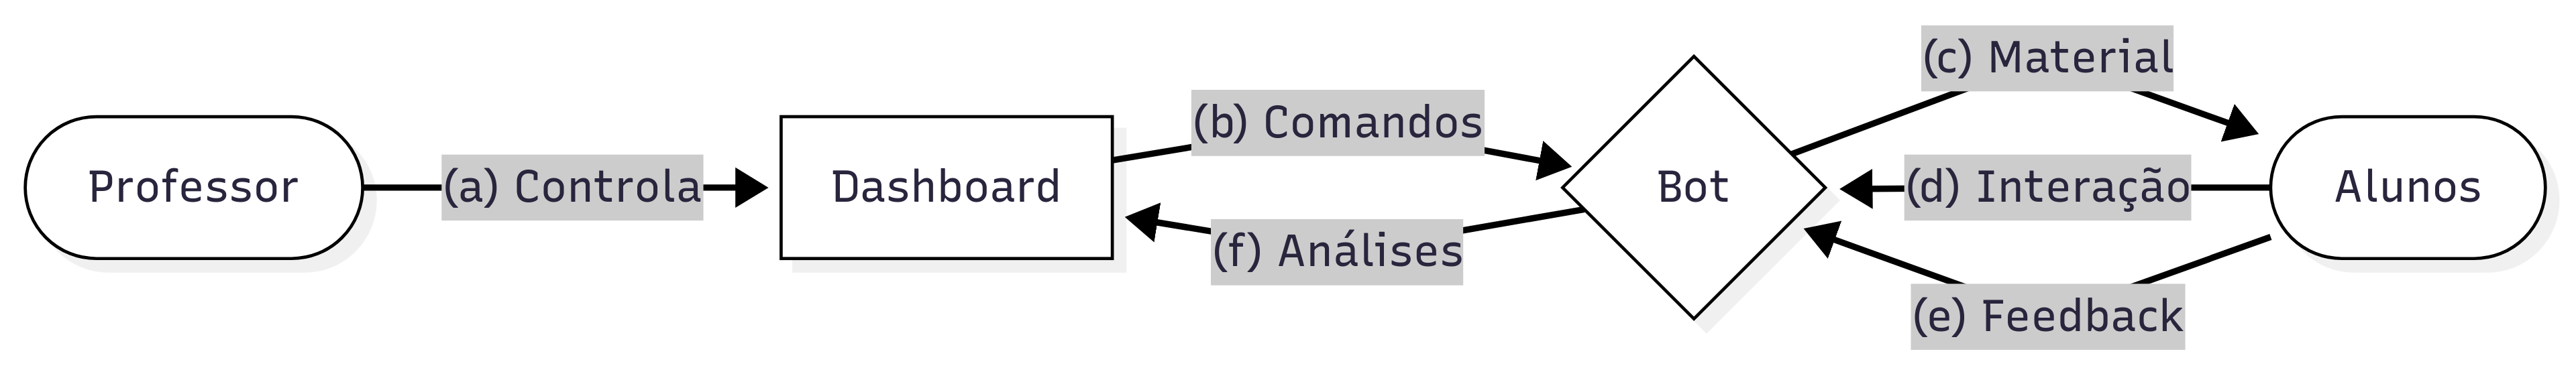
\includegraphics[width=16cm]{modelo-interacao.png}
\caption{Fluxo de interações no ambiente educacional virtual mediado pelo
\textit{bot}. A figura mostra um diagrama com o professor à esquerda, o
\textit{dashboard} do professor como interface de controle, o \textit{bot}
educacional ao centro, e os alunos à direita, ilustrando os fluxos de
comunicação: (a) professor controlando a aula via \textit{dashboard}, (b)
\textit{dashboard} enviando comandos ao \textit{bot}, (c) \textit{bot} 
processando e disponibilizando o material para os alunos, (d) alunos interagindo
com o conteúdo, (e) \textit{bot} coletando \textit{feedback} dos alunos, e (f)
\textit{bot} fornecendo análises em tempo real ao professor através do
\textit{dashboard}.} 
\label{fig:modelo-interacao}
\end{figure}

O modelo de interação implementado neste trabalho fundamenta-se nos três
princípios para interação mediada por \textit{bots} na educação discutidos na
Seção \ref{subsec:principios}: comunicação multidirecional, engajamento ativo e
adaptação contextual. Estes princípios nortearam todo o processo de
\textit{design} e desenvolvimento da solução, garantindo que o \textit{bot}
efetivamente contribua para a implementação de metodologias ativas no ambiente
virtual.

\section{Integração com o Ambiente Educacional}
\label{sec:integracao}

O \textit{bot} foi projetado para se integrar ao Discord, pelos motivos
discutidos na Seção \ref{sec:ferramentas}. A integração sutil com o ambiente
educacional, refere-se à capacidade do \textit{bot} de participar do processo
educacional sem causar rupturas no fluxo natural da aula ou exigir mudanças
drásticas nas práticas pedagógicas já estabelecidas. Essa sutileza manifesta-se
em três dimensões:

\begin{enumerate}
\item \textbf{Presença não-intrusiva}: O \textit{bot} não interrompe a condução
da aula, apenas complementa as atividades quando solicitado ou programado.
\item \textbf{Curva de aprendizado reduzida}: Professores e alunos não precisam
dominar ferramentas complexas, pois as interações ocorrem através de comandos
intuitivos e reações simples.
\item \textbf{Flexibilidade metodológica}: O sistema adapta-se a diferentes
estilos de ensino, não impondo uma abordagem pedagógica específica.
\end{enumerate}

Para materializar esta integração, o sistema também disponibiliza um
\textit{dashboard} específico para uso do professor, como visto em
\ref{subsec:dashboards}, que permite o controle da aula de forma centralizada e
intuitiva, sem a necessidade de comandos complexos ou interrupções no fluxo de
comunicação, como será detalhado na seção \ref{subsec:dashboard}.

\subsection{\textit{Dashboard} do Professor}
\label{subsec:dashboard}

Um elemento chave do sistema é o \textit{dashboard} exclusivo para o professor,
que permite controlar o fluxo da aula sem a necessidade de inserir comandos no
\textit{chat} principal. Este \textit{dashboard} é apresentado como uma
interface web segura, acessível apenas pelo professor, que se comunica com o
\textit{bot} em tempo real. Esta abordagem está diretamente alinhada com o
objetivo de proporcionar uma integração não-invasiva ao fluxo de trabalho
docente, conforme estabelecido na Seção \ref{sec:objetivos} do Capítulo
\ref{cap:revisao}. Através dele, o professor pode:

\begin{itemize}
\item Visualizar estatísticas de engajamento dos alunos em tempo real
\item Controlar a apresentação de slides e materiais didáticos
\item Receber alertas sobre dúvidas e dificuldades dos alunos
\item Lançar atividades interativas e acompanhar seu progresso
\item Obter relatórios detalhados sobre o desempenho da turma
\end{itemize}

Esta abordagem permite que o professor mantenha o controle pedagógico da aula
sem interrupções no fluxo da comunicação, enquanto os alunos interagem
diretamente com o \textit{bot} através de \textit{slash commands} e reações no
ambiente do Discord.

\section{Recursos para Promoção de Metodologias Ativas}
\label{sec:recursos}

O \textit{bot} implementa diversos recursos específicos para viabilizar
metodologias ativas em ambiente remoto. Na seção \ref{subsec:feedback} é
apresentado mecanismos de \textit{feedback} em tempo real que permitem ao
professor avaliar continuamente a compreensão dos alunos, a
\ref{subsec:colaboracao} aborda ferramentas para atividades colaborativas que
incentivam a interação entre os estudantes, e por fim \ref{subsec:pbl} trata das
funcionalidades específicas para aprendizagem baseada em problemas que estimulam
o raciocínio crítico e a resolução de situações práticas.

\subsection{\textit{Feedback} em Tempo Real}
\label{subsec:feedback}

Um dos principais desafios do ensino remoto é perceber as reações dos alunos. O
\textit{bot} permite que os estudantes expressem sua compreensão ou dúvidas
durante a explanação, sem interromper o fluxo da aula, através de:

\begin{itemize}
\item \textbf{Barômetro de compreensão}: Interface visual que agregada as
reações dos alunos
\item \textbf{Alertas de dificuldade}: Notificação ao professor quando um número
significativo de alunos indica não compreender um tópico
\item \textbf{Dúvidas anônimas}: Permite que alunos enviem questões sem
exposição pública
\end{itemize}

\subsection{Atividades Colaborativas}
\label{subsec:colaboracao}

Para fomentar a aprendizagem entre pares, o \textit{bot} oferece:

\begin{itemize}
\item \textbf{Grupos dinâmicos}: Formação automática de equipes para discussão
de tópicos específicos
\item \textbf{Compartilhamento facilitado}: Interface para troca de soluções e
ideias entre alunos
\item \textbf{Revisão coletiva}: Sistema para avaliação colaborativa de
respostas
\end{itemize}

\subsection{Aprendizagem Baseada em Problemas}
\label{subsec:pbl}

A aprendizagem baseada em problemas (vide Seção \ref{cap:intro}) envolve vários
elementos que podem ser incluídos em nosso aplicativo. Dentre esses elementos,
incluímos os seguintes, por serem os mais simples de se implementar:

\begin{itemize}
\item \textbf{Desafios temporizados}: Problemas com tempo definido para
resolução
\item \textbf{Pistas progressivas}: Sugestões que são liberadas gradualmente
durante a resolução
\item \textbf{Compilação e execução de código}: Para disciplinas de programação,
execução segura de códigos submetidos pelos alunos
\end{itemize}

\section{Exemplo Prático: Aula de Comandos de Repetição}
\label{sec:exemplo}

Para ilustrar a aplicação concreta do \textit{bot} em um contexto educacional
real, apresentamos a seguir um cenário baseado em uma aula da disciplina CI1055
- Algoritmos e Estruturas de Dados I, ministrada no Departamento de Informática
da UFPR. O exemplo demonstra como o \textit{bot} auxilia o professor durante uma
aula sobre "Comandos de Repetição" em Pascal. Nas próximas seções, detalharemos
as etapas de preparação da aula pelo professor e as interações que ocorrem
durante a sessão síncrona, evidenciando como os recursos do \textit{bot}
facilitam a implementação das metodologias ativas.

\subsection{Preparação da Aula}
\label{subsec:preparacao}

Antes da aula, o professor utiliza o \textit{dashboard} para preparar o material
didático:

\begin{lstlisting}[
  basicstyle=\ttfamily\footnotesize,
  backgroundcolor=\color{gray!10},
  breaklines=true,
  captionpos=b,
  commentstyle=\color{green!50!black},
  frame=single,
  keywordstyle=\color{blue},
  numbers=left,
  numbersep=5pt,
  numberstyle=\tiny\color{gray},
  stringstyle=\color{red},
  showstringspaces=false,
  tabsize=2
]
[(*@\textit{Dashboard}@*) do Professor]
> Criar Nova Aula
Título: "Comandos de Repetição em Pascal"
Descrição: "Introdução aos comandos de repetição em Pascal com foco no comando while"
Tópicos: "Loops", "Comando while", "Repetição", "Pascal"

> Adicionar Conteúdo
[Título] "Objetivos da aula"
[Conteúdo] "Introduzir conceitos de repetição, apresentar o comando while, 
           resolver exemplos práticos"
[Tipo] Slide

> Adicionar Conteúdo
[Título] "Exemplo inicial: imprimir números de 1 a 5"
[Conteúdo] 
```
program imprimir_de_1_a_5;
begin
  writeln(1);
  writeln(2);
  writeln(3);
  writeln(4);
  writeln(5);
end.
```
[Tipo] Código Pascal

> Configurar Quiz
[Pergunta] "Ao incrementar uma variável dentro de um loop while, 
           qual operação utilizamos em Pascal?"
[Opções] 
- "i := i + 1" (CORRETA)
- "i++"
- "i += 1"
- "increment(i)"
[Tempo] 60 segundos
\end{lstlisting}

O sistema confirma a criação da aula e fornece um código de acesso para os alunos.

\subsection{Interação Durante a Aula}
\label{subsec:interacao}

Durante a aula síncrona, as seguintes interações ocorrem:

\begin{lstlisting}[
  basicstyle=\ttfamily\footnotesize,
  backgroundcolor=\color{gray!10},
  breaklines=true,
  captionpos=b,
  commentstyle=\color{green!50!black},
  frame=single,
  keywordstyle=\color{blue},
  numbers=left,
  numbersep=5pt,
  numberstyle=\tiny\color{gray},
  stringstyle=\color{red},
  showstringspaces=false,
  tabsize=2
]
[(*@\textit{Dashboard}@*) do Professor]
> Iniciar Aula "Comandos de Repetição em Pascal"
Sistema: Aula iniciada. Os alunos podem acessar usando o código #AED1-2310.

> Mostrar Slide 1
Sistema: Exibindo "Objetivos da aula" para todos os participantes.

[Discord - Canal da Aula]
Bot: @everyone O professor iniciou a aula "Comandos de Repetição em Pascal". 
     Use (*@\textit{/participar}@*) para confirmar sua presença.

[Vários alunos utilizam o comando (*@\textit{/participar}@*)]

Professor [no canal de voz]: Vamos começar entendendo por que precisamos de comandos 
                             de repetição. Observem este exemplo inicial no canal.

[(*@\textit{Dashboard}@*) do Professor]
> Mostrar Código "Exemplo inicial"
Sistema: Código exibido no canal #exemplos-de-codigo.

[Discord - Canal #exemplos-de-codigo]
Bot: 
```pascal
program imprimir_de_1_a_5;
begin
  writeln(1);
  writeln(2);
  writeln(3);
  writeln(4);
  writeln(5);
end.
```
Para testar este código, utilize /executar exemplo1

[(*@\textit{Dashboard}@*) do Professor]
> Iniciar Discussão
[Pergunta] "Qual o problema desta abordagem se quisermos imprimir de 1 até 1000?"

[Discord - Canal da Aula]
Bot: DISCUSSÃO: Qual o problema desta abordagem se quisermos imprimir de 1 até 1000?
     Use (*@\textit{/responder}@*) para participar da discussão.

Aluno1: (*@\textit{/responder}@*) Teríamos que escrever mil linhas de código!
Aluno2: (*@\textit{/responder}@*) Código muito repetitivo e difícil de manter.

[(*@\textit{Dashboard}@*) do Professor - Painel de Engajamento]
Status: 15/23 alunos responderam
Participação ativa: 65%
Respostas mais comuns: "código repetitivo" (60%), "muitas linhas" (27%)

[Alguns alunos usam reações no Discord]
[5 alunos reagem com "joinha" (entendi)]
[2 alunos reagem com "?" (tenho dúvida)]

[(*@\textit{Dashboard}@*) do Professor - Alertas]
ATENÇÃO 2 alunos indicaram dúvidas sobre o conceito atual.
Recomendação: Revisitar o conceito com uma abordagem alternativa.

Professor [no canal de voz]: Estou vendo que temos algumas dúvidas. 
                             Vamos revisitar o conceito de forma diferente.

[(*@\textit{Dashboard}@*) do Professor]
> Mostrar Exemplo Interativo
[Título] "Loop while básico"
[Código]
```pascal
program exemplo;
var i: integer;
begin
  i := 1;
  while i <= 5 do
  begin
    writeln(i);
    i := i + 1;
  end;
end.
```
[Opções] Ativar execução por alunos

[Discord - Canal #exemplos-de-codigo]
Bot: EXEMPLO INTERATIVO: Loop while básico
```pascal
program exemplo;
var i: integer;
begin
  i := 1;
  while i <= 5 do
  begin
    writeln(i);
    i := i + 1;
  end;
end.
```
Use /executar para ver o resultado deste código.

Aluno5: /executar
Bot: 
```
1
2
3
4
5
```

Aluno8: /duvida O que acontece se eu esquecer de incrementar i dentro do loop?
Bot: @Professor Dúvida enviada anonimamente: "O que acontece se eu esquecer de incrementar i dentro do loop?"

[(*@\textit{Dashboard}@*) do Professor]
> Responder Dúvida
[Criar Exemplo] "Loop infinito"
```pascal
program loop_infinito;
var i: integer;
begin
  i := 1;
  while i <= 5 do
  begin
    writeln(i);
    // i não é incrementado
  end;
end.
```

[Discord - Canal #exemplos-de-codigo]
Bot: Resposta à dúvida: O que acontece se esquecer de incrementar i
```pascal
program loop_infinito;
var i: integer;
begin
  i := 1;
  while i <= 5 do
  begin
    writeln(i);
    // i não é incrementado
  end;
end.
```
Aviso: O código acima contém um loop infinito. A execução seria interrompida após 
repetir o mesmo valor várias vezes:
```
1
1
1
1
...
```

[(*@\textit{Dashboard}@*) do Professor]
> Criar Desafio
[Título] "Números pares"
[Descrição] "Escreva um programa que leia um número n e imprima todos os números pares de 2 até n"
[Tempo] 10 minutos
[Testes Automáticos] 
- Entrada: "10" | Saída esperada: "2 4 6 8 10"
- Entrada: "7" | Saída esperada: "2 4 6"

[Discord - Canal #desafios]
Bot: NOVO DESAFIO: Números pares
Escreva um programa que leia um número n e imprima todos os números pares de 2 até n.
Tempo: 10 minutos
Use /iniciar-desafio para começar a resolver.

[Vários alunos utilizam o comando /iniciar-desafio, recebendo acesso a canais privados para resolver o problema]

[(*@\textit{Dashboard}@*) do Professor - Monitor de Progresso]
15/23 alunos iniciaram o desafio
8/23 já submeteram soluções
6/23 passaram em todos os testes

[Após o tempo definido]
[(*@\textit{Dashboard}@*) do Professor]
> Encerrar Desafio
> Compartilhar Solução Anônima [ID: 3]

[Discord - Canal #desafios]
Bot: O tempo para o desafio "Números pares" encerrou!
Estatísticas:
- 19/23 alunos participaram
- 15/19 completaram o desafio com sucesso

Solução compartilhada (anônima):
```pascal
program numeros_pares;
var i, n: integer;
begin
  read(n);
  i := 2;
  while i <= n do
  begin
    writeln(i);
    i := i + 2;
  end;
end.
```

[(*@\textit{Dashboard}@*) do Professor]
> Encerrar Aula
> Gerar Relatório

[Discord - Canal da Aula]
Bot: Esta aula foi encerrada. Um resumo das atividades foi enviado ao professor.
     Todo o material continua disponível para consulta nos canais respectivos.

[(*@\textit{E-mail}@*) do Professor - Relatório Automático]
Resumo da aula: "Comandos de Repetição em Pascal"
- Participação: 23/25 alunos ativos (92%)
- Média de interações por aluno: 7.2
- Tópicos com mais dúvidas: "loop infinito" (5 menções), "incremento de variáveis" (3 menções)
- Desafio "Números pares": 19/23 participaram, 15/19 completaram com sucesso
- Alunos com participação abaixo do esperado: 2 (lista anexa)
- Recomendação: Reforçar o conceito de incremento de variáveis na próxima aula
\end{lstlisting}

\chapter{\textit{Bot} Educacional para Metodologias Ativas em Ambientes
Virtuais}
\label{cap:bot}

% Usar o graphicspath para buscar figuras no subdiretório figuras
\graphicspath{\currfiledir/figuras/}

Este capítulo apresenta a concepção do \textit{bot} educacional desenvolvido
neste trabalho, sua arquitetura funcional e como ele se integra ao ambiente de
ensino remoto para facilitar metodologias ativas. Para ilustrar a aplicação
prática, utilizaremos um exemplo concreto baseado em uma aula de programação da
disciplina CI1055 (Algoritmos e Estruturas de Dados I) do DINF da UFPR
\cite{ufpr2021ci1055}.

\section{Visão Conceitual da Aplicação}
\label{sec:visao}

O \textit{bot} educacional proposto foi concebido como um mediador de interações
em ambientes virtuais de aprendizagem, especificamente voltado para facilitar a
implementação de metodologias ativas durante sessões de ensino remoto. O sistema
atua como uma ponte entre professor e alunos, promovendo trocas mais naturais de
informações e \textit{feedback}.

A Figura a seguir ilustra o modelo conceitual de interação entre os
participantes do processo educacional mediado pelo \textit{bot}:

\begin{figure}[htb]
\centering
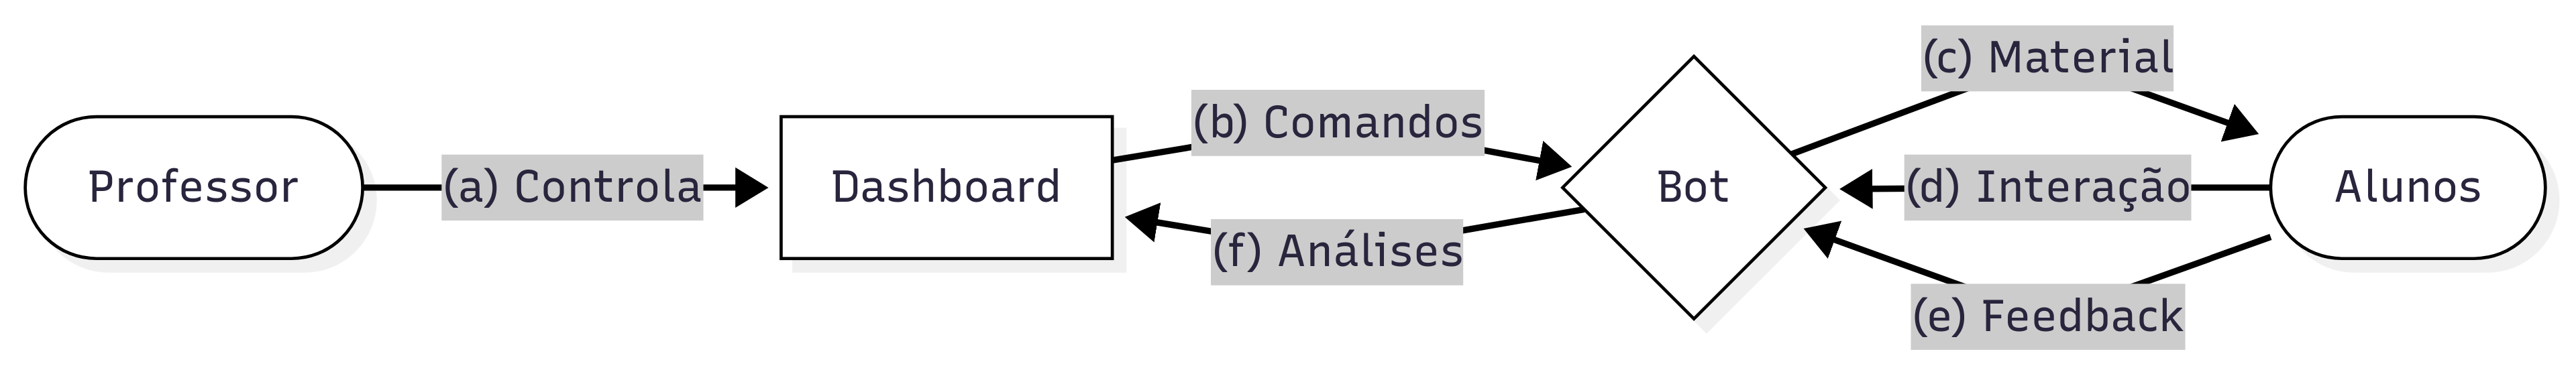
\includegraphics[width=16cm]{modelo-interacao.png}
\caption{Fluxo de interações no ambiente educacional virtual mediado pelo
\textit{bot}. A figura mostra um diagrama com o professor à esquerda, o
\textit{dashboard} do professor como interface de controle, o \textit{bot}
educacional ao centro, e os alunos à direita, ilustrando os fluxos de
comunicação: (a) professor controlando a aula via \textit{dashboard}, (b)
\textit{dashboard} enviando comandos ao \textit{bot}, (c) \textit{bot} 
processando e disponibilizando o material para os alunos, (d) alunos interagindo
com o conteúdo, (e) \textit{bot} coletando \textit{feedback} dos alunos, e (f)
\textit{bot} fornecendo análises em tempo real ao professor através do
\textit{dashboard}.} 
\label{fig:modelo-interacao}
\end{figure}

O modelo de interação implementado neste trabalho fundamenta-se nos três
princípios para interação mediada por \textit{bots} na educação discutidos na
Seção \ref{subsec:principios}: comunicação multidirecional, engajamento ativo e
adaptação contextual. Estes princípios nortearam todo o processo de
\textit{design} e desenvolvimento da solução, garantindo que o \textit{bot}
efetivamente contribua para a implementação de metodologias ativas no ambiente
virtual.

\section{Integração com o Ambiente Educacional}
\label{sec:integracao}

O \textit{bot} foi projetado para se integrar ao Discord, pelos motivos
discutidos na Seção \ref{sec:ferramentas}. A integração sutil com o ambiente
educacional, refere-se à capacidade do \textit{bot} de participar do processo
educacional sem causar rupturas no fluxo natural da aula ou exigir mudanças
drásticas nas práticas pedagógicas já estabelecidas. Essa sutileza manifesta-se
em três dimensões:

\begin{enumerate}
\item \textbf{Presença não-intrusiva}: O \textit{bot} não interrompe a condução
da aula, apenas complementa as atividades quando solicitado ou programado.
\item \textbf{Curva de aprendizado reduzida}: Professores e alunos não precisam
dominar ferramentas complexas, pois as interações ocorrem através de comandos
intuitivos e reações simples.
\item \textbf{Flexibilidade metodológica}: O sistema adapta-se a diferentes
estilos de ensino, não impondo uma abordagem pedagógica específica.
\end{enumerate}

Para materializar esta integração, o sistema também disponibiliza um
\textit{dashboard} específico para uso do professor, como visto em
\ref{subsec:dashboards}, que permite o controle da aula de forma centralizada e
intuitiva, sem a necessidade de comandos complexos ou interrupções no fluxo de
comunicação, como será detalhado na seção \ref{subsec:dashboard}.

\subsection{\textit{Dashboard} do Professor}
\label{subsec:dashboard}

Um elemento chave do sistema é o \textit{dashboard} exclusivo para o professor,
que permite controlar o fluxo da aula sem a necessidade de inserir comandos no
\textit{chat} principal. Este \textit{dashboard} é apresentado como uma
interface web segura, acessível apenas pelo professor, que se comunica com o
\textit{bot} em tempo real. Esta abordagem está diretamente alinhada com o
objetivo de proporcionar uma integração não-invasiva ao fluxo de trabalho
docente, conforme estabelecido na Seção \ref{sec:objetivos} do Capítulo
\ref{cap:revisao}. Através dele, o professor pode:

\begin{itemize}
\item Visualizar estatísticas de engajamento dos alunos em tempo real
\item Controlar a apresentação de slides e materiais didáticos
\item Receber alertas sobre dúvidas e dificuldades dos alunos
\item Lançar atividades interativas e acompanhar seu progresso
\item Obter relatórios detalhados sobre o desempenho da turma
\end{itemize}

Esta abordagem permite que o professor mantenha o controle pedagógico da aula
sem interrupções no fluxo da comunicação, enquanto os alunos interagem
diretamente com o \textit{bot} através de \textit{slash commands} e reações no
ambiente do Discord.

\section{Recursos para Promoção de Metodologias Ativas}
\label{sec:recursos}

O \textit{bot} implementa diversos recursos específicos para viabilizar
metodologias ativas em ambiente remoto. Na seção \ref{subsec:feedback} é
apresentado mecanismos de \textit{feedback} em tempo real que permitem ao
professor avaliar continuamente a compreensão dos alunos, a
\ref{subsec:colaboracao} aborda ferramentas para atividades colaborativas que
incentivam a interação entre os estudantes, e por fim \ref{subsec:pbl} trata das
funcionalidades específicas para aprendizagem baseada em problemas que estimulam
o raciocínio crítico e a resolução de situações práticas.

\subsection{\textit{Feedback} em Tempo Real}
\label{subsec:feedback}

Um dos principais desafios do ensino remoto é perceber as reações dos alunos. O
\textit{bot} permite que os estudantes expressem sua compreensão ou dúvidas
durante a explanação, sem interromper o fluxo da aula, através de:

\begin{itemize}
\item \textbf{Barômetro de compreensão}: Interface visual que agregada as
reações dos alunos
\item \textbf{Alertas de dificuldade}: Notificação ao professor quando um número
significativo de alunos indica não compreender um tópico
\item \textbf{Dúvidas anônimas}: Permite que alunos enviem questões sem
exposição pública
\end{itemize}

\subsection{Atividades Colaborativas}
\label{subsec:colaboracao}

Para fomentar a aprendizagem entre pares, o \textit{bot} oferece:

\begin{itemize}
\item \textbf{Grupos dinâmicos}: Formação automática de equipes para discussão
de tópicos específicos
\item \textbf{Compartilhamento facilitado}: Interface para troca de soluções e
ideias entre alunos
\item \textbf{Revisão coletiva}: Sistema para avaliação colaborativa de
respostas
\end{itemize}

\subsection{Aprendizagem Baseada em Problemas}
\label{subsec:pbl}

A aprendizagem baseada em problemas (vide Seção \ref{cap:intro}) envolve vários
elementos que podem ser incluídos em nosso aplicativo. Dentre esses elementos,
incluímos os seguintes, por serem os mais simples de se implementar:

\begin{itemize}
\item \textbf{Desafios temporizados}: Problemas com tempo definido para
resolução
\item \textbf{Pistas progressivas}: Sugestões que são liberadas gradualmente
durante a resolução
\item \textbf{Compilação e execução de código}: Para disciplinas de programação,
execução segura de códigos submetidos pelos alunos
\end{itemize}

\section{Exemplo Prático: Aula de Comandos de Repetição}
\label{sec:exemplo}

Para ilustrar a aplicação concreta do \textit{bot} em um contexto educacional
real, apresentamos a seguir um cenário baseado em uma aula da disciplina CI1055
- Algoritmos e Estruturas de Dados I, ministrada no Departamento de Informática
da UFPR. O exemplo demonstra como o \textit{bot} auxilia o professor durante uma
aula sobre "Comandos de Repetição" em Pascal. Nas próximas seções, detalharemos
as etapas de preparação da aula pelo professor e as interações que ocorrem
durante a sessão síncrona, evidenciando como os recursos do \textit{bot}
facilitam a implementação das metodologias ativas.

\subsection{Preparação da Aula}
\label{subsec:preparacao}

Antes da aula, o professor utiliza o \textit{dashboard} para preparar o material
didático:

\begin{lstlisting}[
  basicstyle=\ttfamily\footnotesize,
  backgroundcolor=\color{gray!10},
  breaklines=true,
  captionpos=b,
  commentstyle=\color{green!50!black},
  frame=single,
  keywordstyle=\color{blue},
  numbers=left,
  numbersep=5pt,
  numberstyle=\tiny\color{gray},
  stringstyle=\color{red},
  showstringspaces=false,
  tabsize=2
]
[(*@\textit{Dashboard}@*) do Professor]
> Criar Nova Aula
Título: "Comandos de Repetição em Pascal"
Descrição: "Introdução aos comandos de repetição em Pascal com foco no comando while"
Tópicos: "Loops", "Comando while", "Repetição", "Pascal"

> Adicionar Conteúdo
[Título] "Objetivos da aula"
[Conteúdo] "Introduzir conceitos de repetição, apresentar o comando while, 
           resolver exemplos práticos"
[Tipo] Slide

> Adicionar Conteúdo
[Título] "Exemplo inicial: imprimir números de 1 a 5"
[Conteúdo] 
```
program imprimir_de_1_a_5;
begin
  writeln(1);
  writeln(2);
  writeln(3);
  writeln(4);
  writeln(5);
end.
```
[Tipo] Código Pascal

> Configurar Quiz
[Pergunta] "Ao incrementar uma variável dentro de um loop while, 
           qual operação utilizamos em Pascal?"
[Opções] 
- "i := i + 1" (CORRETA)
- "i++"
- "i += 1"
- "increment(i)"
[Tempo] 60 segundos
\end{lstlisting}

O sistema confirma a criação da aula e fornece um código de acesso para os alunos.

\subsection{Interação Durante a Aula}
\label{subsec:interacao}

Durante a aula síncrona, as seguintes interações ocorrem:

\begin{lstlisting}[
  basicstyle=\ttfamily\footnotesize,
  backgroundcolor=\color{gray!10},
  breaklines=true,
  captionpos=b,
  commentstyle=\color{green!50!black},
  frame=single,
  keywordstyle=\color{blue},
  numbers=left,
  numbersep=5pt,
  numberstyle=\tiny\color{gray},
  stringstyle=\color{red},
  showstringspaces=false,
  tabsize=2
]
[(*@\textit{Dashboard}@*) do Professor]
> Iniciar Aula "Comandos de Repetição em Pascal"
Sistema: Aula iniciada. Os alunos podem acessar usando o código #AED1-2310.

> Mostrar Slide 1
Sistema: Exibindo "Objetivos da aula" para todos os participantes.

[Discord - Canal da Aula]
Bot: @everyone O professor iniciou a aula "Comandos de Repetição em Pascal". 
     Use (*@\textit{/participar}@*) para confirmar sua presença.

[Vários alunos utilizam o comando (*@\textit{/participar}@*)]

Professor [no canal de voz]: Vamos começar entendendo por que precisamos de comandos 
                             de repetição. Observem este exemplo inicial no canal.

[(*@\textit{Dashboard}@*) do Professor]
> Mostrar Código "Exemplo inicial"
Sistema: Código exibido no canal #exemplos-de-codigo.

[Discord - Canal #exemplos-de-codigo]
Bot: 
```pascal
program imprimir_de_1_a_5;
begin
  writeln(1);
  writeln(2);
  writeln(3);
  writeln(4);
  writeln(5);
end.
```
Para testar este código, utilize /executar exemplo1

[(*@\textit{Dashboard}@*) do Professor]
> Iniciar Discussão
[Pergunta] "Qual o problema desta abordagem se quisermos imprimir de 1 até 1000?"

[Discord - Canal da Aula]
Bot: DISCUSSÃO: Qual o problema desta abordagem se quisermos imprimir de 1 até 1000?
     Use (*@\textit{/responder}@*) para participar da discussão.

Aluno1: (*@\textit{/responder}@*) Teríamos que escrever mil linhas de código!
Aluno2: (*@\textit{/responder}@*) Código muito repetitivo e difícil de manter.

[(*@\textit{Dashboard}@*) do Professor - Painel de Engajamento]
Status: 15/23 alunos responderam
Participação ativa: 65%
Respostas mais comuns: "código repetitivo" (60%), "muitas linhas" (27%)

[Alguns alunos usam reações no Discord]
[5 alunos reagem com "joinha" (entendi)]
[2 alunos reagem com "?" (tenho dúvida)]

[(*@\textit{Dashboard}@*) do Professor - Alertas]
ATENÇÃO 2 alunos indicaram dúvidas sobre o conceito atual.
Recomendação: Revisitar o conceito com uma abordagem alternativa.

Professor [no canal de voz]: Estou vendo que temos algumas dúvidas. 
                             Vamos revisitar o conceito de forma diferente.

[(*@\textit{Dashboard}@*) do Professor]
> Mostrar Exemplo Interativo
[Título] "Loop while básico"
[Código]
```pascal
program exemplo;
var i: integer;
begin
  i := 1;
  while i <= 5 do
  begin
    writeln(i);
    i := i + 1;
  end;
end.
```
[Opções] Ativar execução por alunos

[Discord - Canal #exemplos-de-codigo]
Bot: EXEMPLO INTERATIVO: Loop while básico
```pascal
program exemplo;
var i: integer;
begin
  i := 1;
  while i <= 5 do
  begin
    writeln(i);
    i := i + 1;
  end;
end.
```
Use /executar para ver o resultado deste código.

Aluno5: /executar
Bot: 
```
1
2
3
4
5
```

Aluno8: /duvida O que acontece se eu esquecer de incrementar i dentro do loop?
Bot: @Professor Dúvida enviada anonimamente: "O que acontece se eu esquecer de incrementar i dentro do loop?"

[(*@\textit{Dashboard}@*) do Professor]
> Responder Dúvida
[Criar Exemplo] "Loop infinito"
```pascal
program loop_infinito;
var i: integer;
begin
  i := 1;
  while i <= 5 do
  begin
    writeln(i);
    // i não é incrementado
  end;
end.
```

[Discord - Canal #exemplos-de-codigo]
Bot: Resposta à dúvida: O que acontece se esquecer de incrementar i
```pascal
program loop_infinito;
var i: integer;
begin
  i := 1;
  while i <= 5 do
  begin
    writeln(i);
    // i não é incrementado
  end;
end.
```
Aviso: O código acima contém um loop infinito. A execução seria interrompida após 
repetir o mesmo valor várias vezes:
```
1
1
1
1
...
```

[(*@\textit{Dashboard}@*) do Professor]
> Criar Desafio
[Título] "Números pares"
[Descrição] "Escreva um programa que leia um número n e imprima todos os números pares de 2 até n"
[Tempo] 10 minutos
[Testes Automáticos] 
- Entrada: "10" | Saída esperada: "2 4 6 8 10"
- Entrada: "7" | Saída esperada: "2 4 6"

[Discord - Canal #desafios]
Bot: NOVO DESAFIO: Números pares
Escreva um programa que leia um número n e imprima todos os números pares de 2 até n.
Tempo: 10 minutos
Use /iniciar-desafio para começar a resolver.

[Vários alunos utilizam o comando /iniciar-desafio, recebendo acesso a canais privados para resolver o problema]

[(*@\textit{Dashboard}@*) do Professor - Monitor de Progresso]
15/23 alunos iniciaram o desafio
8/23 já submeteram soluções
6/23 passaram em todos os testes

[Após o tempo definido]
[(*@\textit{Dashboard}@*) do Professor]
> Encerrar Desafio
> Compartilhar Solução Anônima [ID: 3]

[Discord - Canal #desafios]
Bot: O tempo para o desafio "Números pares" encerrou!
Estatísticas:
- 19/23 alunos participaram
- 15/19 completaram o desafio com sucesso

Solução compartilhada (anônima):
```pascal
program numeros_pares;
var i, n: integer;
begin
  read(n);
  i := 2;
  while i <= n do
  begin
    writeln(i);
    i := i + 2;
  end;
end.
```

[(*@\textit{Dashboard}@*) do Professor]
> Encerrar Aula
> Gerar Relatório

[Discord - Canal da Aula]
Bot: Esta aula foi encerrada. Um resumo das atividades foi enviado ao professor.
     Todo o material continua disponível para consulta nos canais respectivos.

[(*@\textit{E-mail}@*) do Professor - Relatório Automático]
Resumo da aula: "Comandos de Repetição em Pascal"
- Participação: 23/25 alunos ativos (92%)
- Média de interações por aluno: 7.2
- Tópicos com mais dúvidas: "loop infinito" (5 menções), "incremento de variáveis" (3 menções)
- Desafio "Números pares": 19/23 participaram, 15/19 completaram com sucesso
- Alunos com participação abaixo do esperado: 2 (lista anexa)
- Recomendação: Reforçar o conceito de incremento de variáveis na próxima aula
\end{lstlisting}


%=====================================================

\end{document}

%=====================================================
